\documentclass[]{article}
\usepackage{lmodern}
\usepackage{amssymb,amsmath}
\usepackage{ifxetex,ifluatex}
\usepackage{fixltx2e} % provides \textsubscript
\ifnum 0\ifxetex 1\fi\ifluatex 1\fi=0 % if pdftex
  \usepackage[T1]{fontenc}
  \usepackage[utf8]{inputenc}
\else % if luatex or xelatex
  \ifxetex
    \usepackage{mathspec}
  \else
    \usepackage{fontspec}
  \fi
  \defaultfontfeatures{Ligatures=TeX,Scale=MatchLowercase}
\fi
% use upquote if available, for straight quotes in verbatim environments
\IfFileExists{upquote.sty}{\usepackage{upquote}}{}
% use microtype if available
\IfFileExists{microtype.sty}{%
\usepackage{microtype}
\UseMicrotypeSet[protrusion]{basicmath} % disable protrusion for tt fonts
}{}
\usepackage[margin=1in]{geometry}
\usepackage{hyperref}
\hypersetup{unicode=true,
            pdftitle={Analysis of E. coli Time Course RNA-Seq Data},
            pdfauthor={Ethan Ashby, Annie Cohen, Lian Morales, Prof.~Jo Hardin, Prof.~Dan Stoebel, Prof.~Danae Schulz},
            pdfborder={0 0 0},
            breaklinks=true}
\urlstyle{same}  % don't use monospace font for urls
\usepackage{color}
\usepackage{fancyvrb}
\newcommand{\VerbBar}{|}
\newcommand{\VERB}{\Verb[commandchars=\\\{\}]}
\DefineVerbatimEnvironment{Highlighting}{Verbatim}{commandchars=\\\{\}}
% Add ',fontsize=\small' for more characters per line
\usepackage{framed}
\definecolor{shadecolor}{RGB}{248,248,248}
\newenvironment{Shaded}{\begin{snugshade}}{\end{snugshade}}
\newcommand{\KeywordTok}[1]{\textcolor[rgb]{0.13,0.29,0.53}{\textbf{#1}}}
\newcommand{\DataTypeTok}[1]{\textcolor[rgb]{0.13,0.29,0.53}{#1}}
\newcommand{\DecValTok}[1]{\textcolor[rgb]{0.00,0.00,0.81}{#1}}
\newcommand{\BaseNTok}[1]{\textcolor[rgb]{0.00,0.00,0.81}{#1}}
\newcommand{\FloatTok}[1]{\textcolor[rgb]{0.00,0.00,0.81}{#1}}
\newcommand{\ConstantTok}[1]{\textcolor[rgb]{0.00,0.00,0.00}{#1}}
\newcommand{\CharTok}[1]{\textcolor[rgb]{0.31,0.60,0.02}{#1}}
\newcommand{\SpecialCharTok}[1]{\textcolor[rgb]{0.00,0.00,0.00}{#1}}
\newcommand{\StringTok}[1]{\textcolor[rgb]{0.31,0.60,0.02}{#1}}
\newcommand{\VerbatimStringTok}[1]{\textcolor[rgb]{0.31,0.60,0.02}{#1}}
\newcommand{\SpecialStringTok}[1]{\textcolor[rgb]{0.31,0.60,0.02}{#1}}
\newcommand{\ImportTok}[1]{#1}
\newcommand{\CommentTok}[1]{\textcolor[rgb]{0.56,0.35,0.01}{\textit{#1}}}
\newcommand{\DocumentationTok}[1]{\textcolor[rgb]{0.56,0.35,0.01}{\textbf{\textit{#1}}}}
\newcommand{\AnnotationTok}[1]{\textcolor[rgb]{0.56,0.35,0.01}{\textbf{\textit{#1}}}}
\newcommand{\CommentVarTok}[1]{\textcolor[rgb]{0.56,0.35,0.01}{\textbf{\textit{#1}}}}
\newcommand{\OtherTok}[1]{\textcolor[rgb]{0.56,0.35,0.01}{#1}}
\newcommand{\FunctionTok}[1]{\textcolor[rgb]{0.00,0.00,0.00}{#1}}
\newcommand{\VariableTok}[1]{\textcolor[rgb]{0.00,0.00,0.00}{#1}}
\newcommand{\ControlFlowTok}[1]{\textcolor[rgb]{0.13,0.29,0.53}{\textbf{#1}}}
\newcommand{\OperatorTok}[1]{\textcolor[rgb]{0.81,0.36,0.00}{\textbf{#1}}}
\newcommand{\BuiltInTok}[1]{#1}
\newcommand{\ExtensionTok}[1]{#1}
\newcommand{\PreprocessorTok}[1]{\textcolor[rgb]{0.56,0.35,0.01}{\textit{#1}}}
\newcommand{\AttributeTok}[1]{\textcolor[rgb]{0.77,0.63,0.00}{#1}}
\newcommand{\RegionMarkerTok}[1]{#1}
\newcommand{\InformationTok}[1]{\textcolor[rgb]{0.56,0.35,0.01}{\textbf{\textit{#1}}}}
\newcommand{\WarningTok}[1]{\textcolor[rgb]{0.56,0.35,0.01}{\textbf{\textit{#1}}}}
\newcommand{\AlertTok}[1]{\textcolor[rgb]{0.94,0.16,0.16}{#1}}
\newcommand{\ErrorTok}[1]{\textcolor[rgb]{0.64,0.00,0.00}{\textbf{#1}}}
\newcommand{\NormalTok}[1]{#1}
\usepackage{graphicx,grffile}
\makeatletter
\def\maxwidth{\ifdim\Gin@nat@width>\linewidth\linewidth\else\Gin@nat@width\fi}
\def\maxheight{\ifdim\Gin@nat@height>\textheight\textheight\else\Gin@nat@height\fi}
\makeatother
% Scale images if necessary, so that they will not overflow the page
% margins by default, and it is still possible to overwrite the defaults
% using explicit options in \includegraphics[width, height, ...]{}
\setkeys{Gin}{width=\maxwidth,height=\maxheight,keepaspectratio}
\IfFileExists{parskip.sty}{%
\usepackage{parskip}
}{% else
\setlength{\parindent}{0pt}
\setlength{\parskip}{6pt plus 2pt minus 1pt}
}
\setlength{\emergencystretch}{3em}  % prevent overfull lines
\providecommand{\tightlist}{%
  \setlength{\itemsep}{0pt}\setlength{\parskip}{0pt}}
\setcounter{secnumdepth}{0}
% Redefines (sub)paragraphs to behave more like sections
\ifx\paragraph\undefined\else
\let\oldparagraph\paragraph
\renewcommand{\paragraph}[1]{\oldparagraph{#1}\mbox{}}
\fi
\ifx\subparagraph\undefined\else
\let\oldsubparagraph\subparagraph
\renewcommand{\subparagraph}[1]{\oldsubparagraph{#1}\mbox{}}
\fi

%%% Use protect on footnotes to avoid problems with footnotes in titles
\let\rmarkdownfootnote\footnote%
\def\footnote{\protect\rmarkdownfootnote}

%%% Change title format to be more compact
\usepackage{titling}

% Create subtitle command for use in maketitle
\providecommand{\subtitle}[1]{
  \posttitle{
    \begin{center}\large#1\end{center}
    }
}

\setlength{\droptitle}{-2em}

  \title{Analysis of \emph{E. coli} Time Course RNA-Seq Data}
    \pretitle{\vspace{\droptitle}\centering\huge}
  \posttitle{\par}
    \author{Ethan Ashby, Annie Cohen, Lian Morales, Prof.~Jo Hardin, Prof.~Dan
Stoebel, Prof.~Danae Schulz}
    \preauthor{\centering\large\emph}
  \postauthor{\par}
      \predate{\centering\large\emph}
  \postdate{\par}
    \date{9/17/2019}


\begin{document}
\maketitle

\section{Table of Contents}\label{table-of-contents}

\begin{enumerate}
\def\labelenumi{\arabic{enumi}.}
\tightlist
\item
  Introduction\\
  \indent 1.1 Background on \emph{E. coli}\\
  \indent 1.2 RNA-Seq\\
  \indent 1.3 Our data
\item
  Normalization
\item
  Differential Expression\\
  \indent 3.1 DESeq2\\
  \indent 3.2 ImpulseDE2\\
  \indent 3.3 maSigPro\\
  \indent 3.4 Find the intersection
\item
  Visualization\\
  \indent 4.1 Tidying our data\\
  \indent 4.2 ggplot2\\
  \indent 4.3 Shiny App
\item
  Analysis\\
  \indent 5.1 PAM Clustering\\
  \indent 5.2 Gene Ontology Analysis\\
  \indent 5.3 Gene Set Enrichment Analysis
\item
  References
\end{enumerate}

\section{\texorpdfstring{\textbf{1}
Introduction}{1 Introduction}}\label{introduction}

\subsubsection{\texorpdfstring{\textbf{1.1} Background on \emph{E.
coli}}{1.1 Background on E. coli}}\label{background-on-e.-coli}

E. coli possesses a general stress response to a variety of
environmental stresses (Battesti \emph{et al} 2011, Hengge 2011) ranging
from osmotic shock to nutrient starvation. According to preliminary data
from Professor Daniel Stoebel, a key transcription factor coordinating
this response is RpoS, which regulates one quarter of the bacteria's
genome. Simple interpretations of transcriptional networks often invoke
an analogy of an on/off switch, in which the presence of a stimulus
turns some genes on and other genes off. However, these simple
interpretations don't adequately describe the complex, dyanmic processes
underlying many transcriptional responses to stimuli. Currently, there
exists a limited understanding regarding the dynamic nature of
transcriptional responses, and the well-annotated, heavily-studied
genome of E. coli presents an excellent model to study these intricate
regulatory circuits. Past research has determined three different
profiles for genes in relation to RpoS. Linear genes' expression
increases linearly with an increase in RpoS. Genes are considered
sensitive if low levels of RpoS cause them to react more than expected
in the linear profile and insensitive genes are less expressed with low
levels of RpoS than linear genes. This research examines whether genes
that have previously been identified as linear, sensitive, or
insensitive have similar profiles of expression over time under cell
stress conditions.

\subsubsection{\texorpdfstring{\textbf{1.2}
RNA-Seq}{1.2 RNA-Seq}}\label{rna-seq}

RNA-Seq is the process of extracting, fragmenting, amplifying,
sequencing, and mapping RNA to a reference gene in order to determine
gene expression levels. Sequencing of RNA data allows us to determine
how RpoS regulates genes in response to a stressor such as starvation.
We use RNA-Seq to compare the gene expression levels across treatments
and time points. We are interested in both the differences in expression
between our treatment samples, wildtype (WT), and our control (dRpoS or
knockout RpoS), as well as the differential expression of WT from 0 to
150 minutes of starvation.

\subsubsection{\texorpdfstring{\textbf{1.3} Our
data}{1.3 Our data}}\label{our-data}

The data we recieved from Professor Stoebel and his lab was a count
matrix, with 37 columns. The column names specify the strain, timepoint,
treatment, and replicate of the sample. ``JH\_01'' or ``JH\_02''
specifies the strain of \emph{E. coli}, where ``JH\_01'' is the wildtype
under starvation, our treatment, and ``JH\_02'' is delta-RpoS, our
control in which RpoS is removed from the cells, under starvation.
``A'', ``B'', and ``C'' denotes the biological replicate and the number
following it indicates the time point: ``01'' is 0, ``02'' is 30, ``03''
is 60, ``04'' is 90, ``05'' is 120, and ``06'' is 150 minutes. The
original data came with a column called ``Geneid'', which denotes the
specific gene. However, we needed a matrix of only count data in order
to normalize our data, so we assigned this column as the row names and
then deleted the column. In order to compare these genes with external
gene lists, we parse the \texttt{Geneid} column into \texttt{genename},
which is a 3-4 digit character string, usually containing one capital
letter. \(~\)

\begin{Shaded}
\begin{Highlighting}[]
\KeywordTok{head}\NormalTok{(ec_rawcounts[,}\DecValTok{1}\OperatorTok{:}\DecValTok{6}\NormalTok{],}\DecValTok{6}\NormalTok{)}
\end{Highlighting}
\end{Shaded}

\begin{verbatim}
##      JH01_A01 JH01_A02 JH01_A03 JH01_A04 JH01_A05 JH01_A06
## thrL     2761     1599     2451     1994     1055     4025
## thrA     2072      441     1203      739      605     1645
## thrB     1000      278      640      537      606     1349
## thrC     1775      530     1174      762      826     2072
## yaaX      119       36       40       42       28       45
## yaaA      428      424      550      553      265      509
\end{verbatim}

\(~\)

\section{\texorpdfstring{\textbf{2}
Normalization}{2 Normalization}}\label{normalization}

Normalization is an extremely influential step in the process of
determining differentially expressed genes. It is necessary in order to
minimize external factors such as gene length and sequencing depth. If a
gene is longer, there is a higher probability of having more reads
because of its longer sequence. Similarly, if one sample has
disproportionately more reads than another, it will return a false
positive. Therefore, we must normalize for both gene length and
sequencing depth.

We tested out many normalization methods including \texttt{DESeq2} and
\texttt{edgeR}. \texttt{DESeq2} is a normalization and differential
expression analysis method that divides counts by sample specific size
factors that are calculated as the median of the ratios of read counts
to the geometric mean. \texttt{EdgeR} is similarly both a normalization
and differential expression analysis method that employs the trimmed
mean method (TMM), where gene expression is adjusted by a size factor
that takes into account the fold change and relative expression level to
its sample (Ciaran et. al). Through a comparison of size factors, we
determined that the two methods produced very similar normalized counts.
We ultimately decided to use \texttt{DESeq2} because of its abundant
documentation.

\(~\)

\texttt{DESeq2} normalizes data within the differential expression
analysis function pipeline, so we first run the \texttt{DESeq()}
function and then extract the normalized counts.

\begin{Shaded}
\begin{Highlighting}[]
\CommentTok{# Create DESeq dataframe}
\NormalTok{ec_dds <-}\StringTok{ }\KeywordTok{DESeqDataSetFromMatrix}\NormalTok{(ec_rawcounts, }\DataTypeTok{colData =}\NormalTok{ ec_coldata, }
                                 \DataTypeTok{design =} \OperatorTok{~}\StringTok{ }\NormalTok{timetreat)}

\CommentTok{# Run DESeq and extract normalized counts}
\NormalTok{ec_dds_de <-}\StringTok{ }\KeywordTok{DESeq}\NormalTok{(ec_dds)}
\NormalTok{ec_normcounts <-}\StringTok{ }\KeywordTok{as.data.frame}\NormalTok{(}\KeywordTok{counts}\NormalTok{(ec_dds_de, }\DataTypeTok{normalized=}\OtherTok{TRUE}\NormalTok{))}

\KeywordTok{head}\NormalTok{(ec_normcounts[}\DecValTok{1}\OperatorTok{:}\DecValTok{6}\NormalTok{],}\DecValTok{6}\NormalTok{)}
\end{Highlighting}
\end{Shaded}

\begin{verbatim}
##       JH01_A01   JH01_A02   JH01_A03   JH01_A04   JH01_A05   JH01_A06
## thrL 3442.1830 2874.70179 2562.00610 2098.83952 1526.87418 3087.26245
## thrA 2583.1956  792.83520 1257.48402  777.85477  875.60083 1261.75074
## thrB 1246.7160  499.79181  668.98568  565.23411  877.04811 1034.71231
## thrC 2212.9210  952.84049 1227.17061  802.06405 1195.44841 1589.26902
## yaaX  148.3592   64.72124   41.81161   44.20825   40.52367   34.51598
## yaaA  533.5945  762.27239  574.90957  582.07535  383.52764  390.41406
\end{verbatim}

\(~\)

\section{\texorpdfstring{\textbf{3} Differential
Expression}{3 Differential Expression}}\label{differential-expression}

Differential expression measures whether or not the gene expression of
the same gene in different groups or treatments is significantly
different. We apply three different differential expression analysis
methods below to determine a list of differentially expressed genes in
our data se.

\subsubsection{\texorpdfstring{\textbf{3.1}
DESeq2}{3.1 DESeq2}}\label{deseq2}

According to Mistry, Meeta, \emph{et al.} (2017), \texttt{DESeq2}
determines differential expression by:\\
1. Normalization of the raw counts by determining size factors and
adjusting each sample by the size factor.\\
2. Measuring gene-wise dispersions, where dispersion, \(\alpha\),
measures the variability within biological replicates of the same
sample: \(\text {Var} = \mu + \alpha\mu^2\).\\
3. Adjusting dispersion estimates to fit a curve created by the
distribution of dispersion estimates. Use \texttt{plotDispEsts()} to see
fit estimates for yourself.\\
4. Comparing normalized counts with a negative binomial distribution
with the sample mean, \(\mu_j\), and gene-wise dispersion parameter,
\(\alpha_j\) to determine the significance of differential expression.

Because we already ran \texttt{DESeq()} above, we can now extract the
significant results. We chose a p-value of 0.01 to be consistent across
all of our work. \texttt{DESeq2} is a two-sample comparison method, but
we want to accurately determine differentially expressed genes across
\emph{all} the time points. Therefore, we compute:\\
1. A list of differentially expressed genes between the treatment group
(wild-type \emph{E. coli}) at 0 minutes and 150 minutes.\\
2. A list of differentially expressed genes between the treatment group
and the control (delta-RpoS \emph{E. coli}), both at 150 minutes.\\
3. The intersection of the gene lists, or the genes that appear in both
lists, which we use as our differentially expressed gene list from
\texttt{DESeq2}.

\begin{Shaded}
\begin{Highlighting}[]
\KeywordTok{ggplot}\NormalTok{()}
\end{Highlighting}
\end{Shaded}


\includegraphics{EcoliTechnicalReport_files/figure-latex/unnamed-chunk-2-1.pdf}

\begin{Shaded}
\begin{Highlighting}[]
\NormalTok{EC_sig_genes <-}\StringTok{ }\KeywordTok{c}\NormalTok{()}

\CommentTok{# Determine the genes that are differentially expressed between WT0 and WT150}
\NormalTok{de_results <-}\StringTok{ }\KeywordTok{results}\NormalTok{(ec_dds_de, }\DataTypeTok{contrast =} \KeywordTok{c}\NormalTok{(}\StringTok{"timetreat"}\NormalTok{, }\StringTok{"WT150"}\NormalTok{,}\StringTok{"WT0"}\NormalTok{))}
\CommentTok{# Filter for a p-value less than 0.01}
\NormalTok{resSig <-}\StringTok{ }\NormalTok{de_results[ }\KeywordTok{which}\NormalTok{(de_results}\OperatorTok{$}\NormalTok{padj }\OperatorTok{<}\StringTok{ }\FloatTok{0.01}\NormalTok{ ), ]}
\NormalTok{resSig}\OperatorTok{$}\NormalTok{genename <-}\StringTok{ }\KeywordTok{rownames}\NormalTok{(resSig)}
\NormalTok{ind <-}\StringTok{ }\KeywordTok{match}\NormalTok{(}\KeywordTok{rownames}\NormalTok{(ec_normcounts),resSig}\OperatorTok{$}\NormalTok{genename)}
\NormalTok{ec_normcounts}\OperatorTok{$}\NormalTok{sig <-}\StringTok{ }\NormalTok{resSig}\OperatorTok{$}\NormalTok{genename[ind]}
\NormalTok{EC_sig_genes}\OperatorTok{$}\NormalTok{WT_compare <-}\StringTok{ }\NormalTok{ec_normcounts }\OperatorTok
\StringTok{ }\KeywordTok{filter}\NormalTok{(}\OperatorTok{!}\KeywordTok{is.na}\NormalTok{(ec_normcounts}\OperatorTok{$}\NormalTok{sig))}


\CommentTok{# Determine the genes that are differentially expressed between WT150 and dRpoS150}
\NormalTok{de_results <-}\StringTok{ }\KeywordTok{results}\NormalTok{(ec_dds_de, }\DataTypeTok{contrast =} \KeywordTok{c}\NormalTok{(}\StringTok{"timetreat"}\NormalTok{, }\StringTok{"WT150"}\NormalTok{,}\StringTok{"dRpoS150"}\NormalTok{))}
\CommentTok{# Again, filter by p-value.}
\NormalTok{resSig <-}\StringTok{ }\NormalTok{de_results[ }\KeywordTok{which}\NormalTok{(de_results}\OperatorTok{$}\NormalTok{padj }\OperatorTok{<}\StringTok{ }\FloatTok{0.01}\NormalTok{ ), ]}
\NormalTok{resSig}\OperatorTok{$}\NormalTok{genename <-}\StringTok{ }\KeywordTok{rownames}\NormalTok{(resSig)}
\NormalTok{ind <-}\StringTok{ }\KeywordTok{match}\NormalTok{(}\KeywordTok{rownames}\NormalTok{(ec_normcounts),resSig}\OperatorTok{$}\NormalTok{genename)}
\NormalTok{ec_normcounts}\OperatorTok{$}\NormalTok{sig <-}\StringTok{ }\NormalTok{resSig}\OperatorTok{$}\NormalTok{genename[ind]}
\NormalTok{EC_sig_genes}\OperatorTok{$}\NormalTok{treat_compare <-}\StringTok{ }\NormalTok{ec_normcounts }\OperatorTok
\StringTok{ }\KeywordTok{filter}\NormalTok{(}\OperatorTok{!}\KeywordTok{is.na}\NormalTok{(ec_normcounts}\OperatorTok{$}\NormalTok{sig))}

\CommentTok{# Find the intersection of the two lists of differentially expressed genes}
\NormalTok{EC_sig_genes <-}\StringTok{ }\KeywordTok{intersect}\NormalTok{(EC_sig_genes}\OperatorTok{$}\NormalTok{WT_compare}\OperatorTok{$}\NormalTok{sig, EC_sig_genes}\OperatorTok{$}\NormalTok{treat_compare}\OperatorTok{$}\NormalTok{sig)}
\end{Highlighting}
\end{Shaded}

\subsubsection{\texorpdfstring{\textbf{3.2}
ImpulseDE2}{3.2 ImpulseDE2}}\label{impulsede2}

ImpulseDE2 is a serial method for differential expression that models
data based on the impulse model, which has parameters
\(t_1, t_2, h_0, h_1, \text{and } b.\) The impulse model has a spike,
characterized by its beginning height, \(h_0\), inflection point,
\(t_1\), its height, \(h_1\), and its slope at \(t_1\), \(b\). Then the
model decreases into its steady state, characterized by the second
inflection point, \(t_2\), and its final height, \(h_2\).

\begin{figure}
\centering
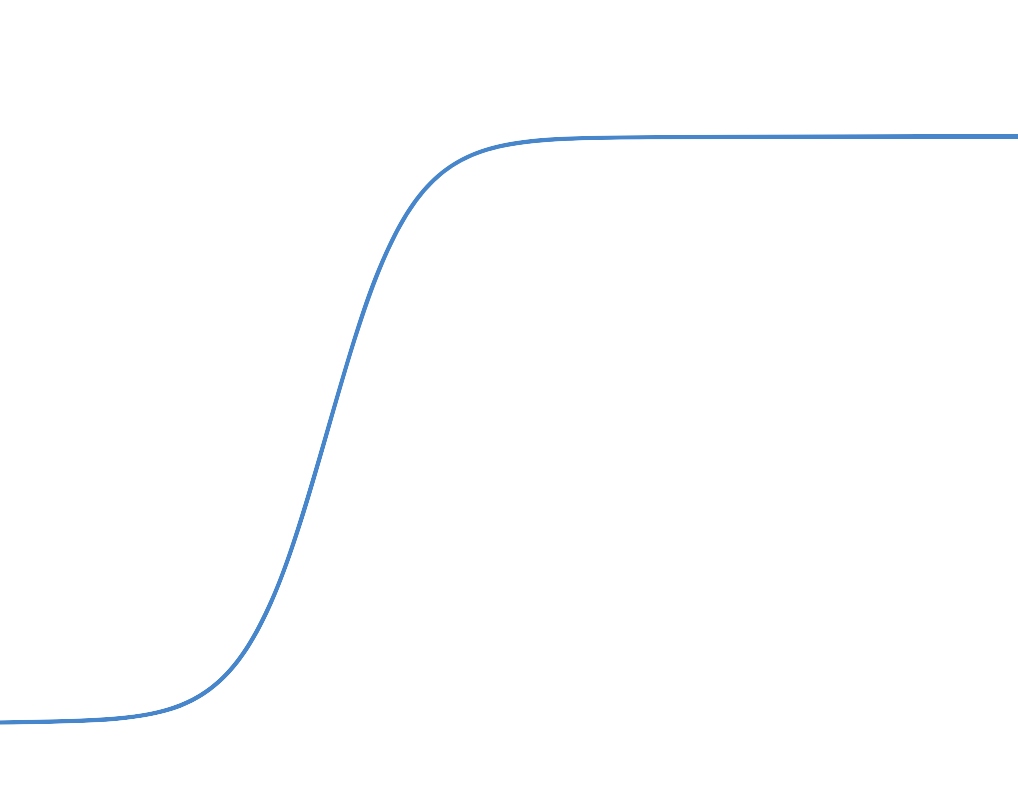
\includegraphics{"/EthanAshby/Sig Model.png"}
\caption{``Sigmoid model of expression has parameters h\_0, the height
of expression at time 0, t, the time at beta, beta, the maximum slope,
and h\_1, the final slope.''}
\end{figure}

According to Fischer et al., ImpulseDE2 determines differential
expression by:\\
\textbf{1.} running DESeq2 and adjusting gene-wise dispersion estimates
from DESeq2 to fit a curve;\\
\textbf{2.} computing size factors and normalizing counts;\\
\textbf{3.} fitting null and alternative model to each of the genes;\\
\textbf{4.} fitting sigmoid model to the treatment condition -- in our
case, samples containing the RpoS translation factor;\\
\textbf{5.} and determining differential expression based on these
models fits to each gene using a log-likelihood ratio (Fischer et al.
2018).

\begin{Shaded}
\begin{Highlighting}[]
\CommentTok{# Set up design matrix}
\NormalTok{ec_design <-}\StringTok{ }\KeywordTok{data.frame}\NormalTok{(}\DataTypeTok{Sample=}\KeywordTok{colnames}\NormalTok{(ec_rawcounts),}
                        \DataTypeTok{Condition=}\KeywordTok{c}\NormalTok{(}\KeywordTok{rep}\NormalTok{(}\StringTok{"case"}\NormalTok{,}\DecValTok{6}\NormalTok{), }\KeywordTok{rep}\NormalTok{(}\StringTok{"control"}\NormalTok{,}\DecValTok{6}\NormalTok{), }\KeywordTok{rep}\NormalTok{(}\StringTok{"case"}\NormalTok{,}\DecValTok{6}\NormalTok{), }
                                    \KeywordTok{rep}\NormalTok{(}\StringTok{"control"}\NormalTok{,}\DecValTok{6}\NormalTok{), }\KeywordTok{rep}\NormalTok{(}\StringTok{"case"}\NormalTok{,}\DecValTok{6}\NormalTok{), }
                                    \KeywordTok{rep}\NormalTok{(}\StringTok{"control"}\NormalTok{,}\DecValTok{6}\NormalTok{)), }
                        \DataTypeTok{Time=}\KeywordTok{rep}\NormalTok{(}\KeywordTok{c}\NormalTok{(}\DecValTok{0}\NormalTok{,}\DecValTok{30}\NormalTok{,}\DecValTok{60}\NormalTok{,}\DecValTok{90}\NormalTok{,}\DecValTok{120}\NormalTok{,}\DecValTok{150}\NormalTok{),}\DecValTok{6}\NormalTok{))}
\end{Highlighting}
\end{Shaded}

\begin{Shaded}
\begin{Highlighting}[]
\CommentTok{# Set `boolCaseCtrl = TRUE` because our data has both case and control conditions, }
\CommentTok{#`scaQThres = 0.01` specifies the level of significance, }
\CommentTok{#`scaNProc = 8` speeds up the function's runtime, }
\CommentTok{#and `boolIdentifyTransients = TRUE` indicates that we are also fitting the sigmoidal model.}
\NormalTok{impulse_ecoli <-}\StringTok{ }\NormalTok{ImpulseDE2}\OperatorTok{::}\KeywordTok{runImpulseDE2}\NormalTok{(}\KeywordTok{as.matrix}\NormalTok{(ec_rawcounts), }
\NormalTok{                                           ec_design, }\DataTypeTok{boolCaseCtrl=}\OtherTok{TRUE}\NormalTok{,}
                                           \DataTypeTok{vecConfounders=}\OtherTok{NULL}\NormalTok{, }\DataTypeTok{scaQThres =} \FloatTok{0.01}\NormalTok{,}
                                           \DataTypeTok{scaNProc =} \DecValTok{8}\NormalTok{, }
                                           \DataTypeTok{boolIdentifyTransients =} \OtherTok{TRUE}\NormalTok{)}
\end{Highlighting}
\end{Shaded}

\subsubsection{\texorpdfstring{\textbf{3.3}
maSigPro}{3.3 maSigPro}}\label{masigpro}

maSigPro is another serial method that determines genes with significant
expression differences over time and between conditions. According to
Conesa and Nueda (2017), the package performs differential expression
analysis by:

\textbf{1.} defining a regression model for the data with the
experimental conditions identified by dummy variables;\\
\textbf{2.} using least-squared method to adjust the model;\\
\textbf{3.} selecting differentially expressed genes controlling for
false discovery rates;\\
\textbf{4.} and applying stepwise regression to determine differential
expression between groups (Conesa and Nueda 2017).

\begin{Shaded}
\begin{Highlighting}[]
\CommentTok{# Set up design}
\NormalTok{Time <-}\StringTok{ }\KeywordTok{rep}\NormalTok{(}\KeywordTok{c}\NormalTok{(}\DecValTok{0}\NormalTok{,}\DecValTok{30}\NormalTok{,}\DecValTok{60}\NormalTok{,}\DecValTok{90}\NormalTok{,}\DecValTok{120}\NormalTok{,}\DecValTok{150}\NormalTok{),}\DecValTok{6}\NormalTok{)}
\NormalTok{Replicate <-}\StringTok{ }\KeywordTok{rep}\NormalTok{(}\DecValTok{1}\OperatorTok{:}\DecValTok{3}\NormalTok{, }\DecValTok{12}\NormalTok{)}
\NormalTok{Control <-}\StringTok{ }\KeywordTok{c}\NormalTok{(}\KeywordTok{rep}\NormalTok{(}\DecValTok{0}\NormalTok{, }\DecValTok{6}\NormalTok{), }\KeywordTok{rep}\NormalTok{(}\DecValTok{1}\NormalTok{, }\DecValTok{6}\NormalTok{), }\KeywordTok{rep}\NormalTok{(}\DecValTok{0}\NormalTok{, }\DecValTok{6}\NormalTok{), }\KeywordTok{rep}\NormalTok{(}\DecValTok{1}\NormalTok{, }\DecValTok{6}\NormalTok{), }\KeywordTok{rep}\NormalTok{(}\DecValTok{0}\NormalTok{, }\DecValTok{6}\NormalTok{), }\KeywordTok{rep}\NormalTok{(}\DecValTok{1}\NormalTok{,}\DecValTok{6}\NormalTok{))}
\NormalTok{d_Rpos <-}\StringTok{ }\KeywordTok{c}\NormalTok{(}\KeywordTok{rep}\NormalTok{(}\DecValTok{1}\NormalTok{, }\DecValTok{6}\NormalTok{), }\KeywordTok{rep}\NormalTok{(}\DecValTok{0}\NormalTok{, }\DecValTok{6}\NormalTok{), }\KeywordTok{rep}\NormalTok{(}\DecValTok{1}\NormalTok{, }\DecValTok{6}\NormalTok{), }\KeywordTok{rep}\NormalTok{(}\DecValTok{0}\NormalTok{, }\DecValTok{6}\NormalTok{), }\KeywordTok{rep}\NormalTok{(}\DecValTok{1}\NormalTok{, }\DecValTok{6}\NormalTok{), }\KeywordTok{rep}\NormalTok{(}\DecValTok{0}\NormalTok{, }\DecValTok{6}\NormalTok{))}
\NormalTok{ec_design <-}\StringTok{ }\KeywordTok{cbind}\NormalTok{(Time, Replicate, Control, d_Rpos)}
\KeywordTok{rownames}\NormalTok{(ec_design) <-}\StringTok{ }\KeywordTok{colnames}\NormalTok{(ec_rawcounts)}

\CommentTok{# Get DESeq2 normalized counts and create a design matrix}
\NormalTok{ec_normcounts <-}\StringTok{ }\KeywordTok{as.data.frame}\NormalTok{(}\KeywordTok{counts}\NormalTok{(ec_dds_de, }\DataTypeTok{normalized=}\OtherTok{TRUE}\NormalTok{))}
\NormalTok{ec_design <-}\StringTok{ }\KeywordTok{make.design.matrix}\NormalTok{(ec_design, }\DataTypeTok{degree=}\DecValTok{5}\NormalTok{)}
\end{Highlighting}
\end{Shaded}

\begin{Shaded}
\begin{Highlighting}[]
\CommentTok{# perform a regression fit for our gene expression data. }
\CommentTok{# Set `Q = 0.01` for our significance level, }
\CommentTok{# set `MT.adjust = "BH"` to adjust our p-values using the Benajamini & Holderberg correction method}
\NormalTok{fits <-}\StringTok{ }\KeywordTok{p.vector}\NormalTok{(ec_normcounts, ec_design, }\DataTypeTok{Q=}\FloatTok{0.01}\NormalTok{, }\DataTypeTok{MT.adjust =} \StringTok{"BH"}\NormalTok{, }
                 \DataTypeTok{min.obs=}\DecValTok{6}\NormalTok{, }\DataTypeTok{counts=}\OtherTok{TRUE}\NormalTok{)}

\CommentTok{# perform a stepwise regression fit for our gene expression data.}
\CommentTok{# Set `step.method = "backward"` and `alfa = 0.01` to specify significance level}
\NormalTok{tsep <-}\StringTok{ }\KeywordTok{T.fit}\NormalTok{(fits, }\DataTypeTok{step.method =} \StringTok{"backward"}\NormalTok{, }\DataTypeTok{alfa=}\FloatTok{0.01}\NormalTok{)}

\CommentTok{# Get significant genes between delta_RpoS and Control}
\NormalTok{sigs <-}\StringTok{ }\KeywordTok{get.siggenes}\NormalTok{(tsep, }\DataTypeTok{rsq =} \FloatTok{0.6}\NormalTok{, }\DataTypeTok{vars =} \StringTok{"groups"}\NormalTok{)}
\NormalTok{maSigProGenes <-}\StringTok{ }\NormalTok{sigs}\OperatorTok{$}\NormalTok{summary}\OperatorTok{$}\NormalTok{d_RposvsControl}
\end{Highlighting}
\end{Shaded}

\subsubsection{\texorpdfstring{\textbf{3.4} Find the
Intersection}{3.4 Find the Intersection}}\label{find-the-intersection}

In order to balance our sensitivity with false discovery rates, we
decided to consider genes differentially expressed if they were
identified in at least 2 of the 3 methods.

First, we made lists of genes from all of the combinations of
intersections between each method and then took the union of that list.

\begin{Shaded}
\begin{Highlighting}[]
\CommentTok{# Intersect each gene list with another method}
\NormalTok{DS_IM <-}\StringTok{ }\KeywordTok{distinct}\NormalTok{(}\KeywordTok{data.frame}\NormalTok{(}\StringTok{"genename"}\NormalTok{ =}\StringTok{ }\KeywordTok{intersect}\NormalTok{(EC_sig_genes,}
\NormalTok{                                                    impulse_ecoli}\OperatorTok{$}\NormalTok{vecDEGenes)))}
\NormalTok{IM_MA <-}\StringTok{ }\KeywordTok{distinct}\NormalTok{(}\KeywordTok{data.frame}\NormalTok{(}\StringTok{"genename"}\NormalTok{ =}\StringTok{ }\KeywordTok{intersect}\NormalTok{(impulse_ecoli}\OperatorTok{$}\NormalTok{vecDEGenes,}
\NormalTok{                                                    maSigProGenes)))}
\NormalTok{MA_DS <-}\StringTok{ }\KeywordTok{distinct}\NormalTok{(}\KeywordTok{data.frame}\NormalTok{(}\StringTok{"genename"}\NormalTok{ =}\StringTok{ }\KeywordTok{intersect}\NormalTok{(maSigProGenes, EC_sig_genes)))}

\CommentTok{# Take the union of all three of these intersections, making sure to delete duplicate genes.}
\NormalTok{EC_DEGs <-}\StringTok{ }\KeywordTok{distinct}\NormalTok{(}\KeywordTok{bind_rows}\NormalTok{(DS_IM, IM_MA, MA_DS))}
\end{Highlighting}
\end{Shaded}

Next we can visualize this overlap with the \texttt{vennDiagram}
package.

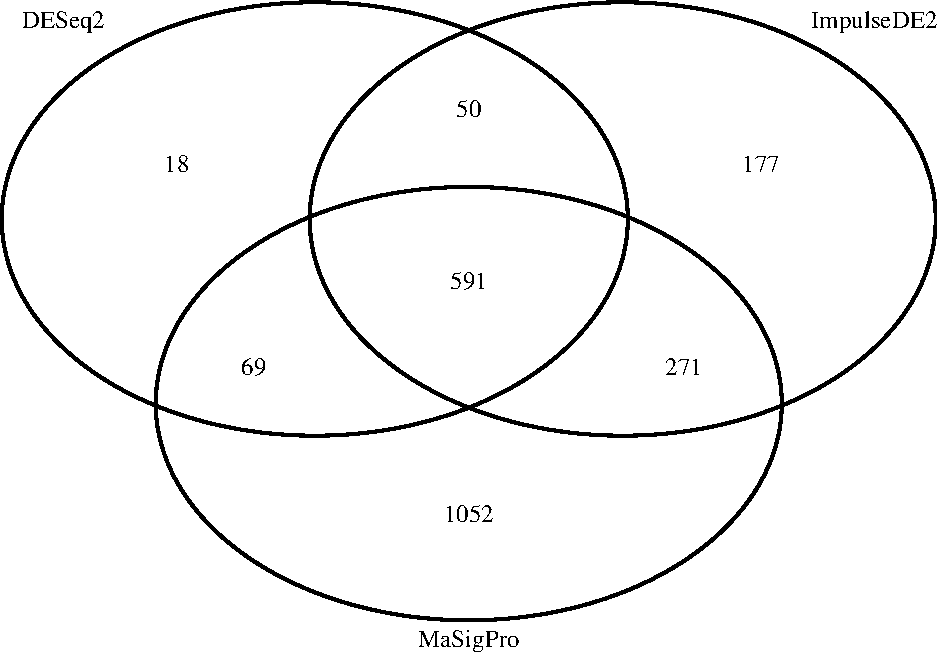
\includegraphics{EcoliTechnicalReport_files/figure-latex/plot intersection-1.pdf}

\begin{verbatim}
## (polygon[GRID.polygon.28], polygon[GRID.polygon.29], polygon[GRID.polygon.30], polygon[GRID.polygon.31], polygon[GRID.polygon.32], polygon[GRID.polygon.33], text[GRID.text.34], text[GRID.text.35], text[GRID.text.36], text[GRID.text.37], text[GRID.text.38], text[GRID.text.39], text[GRID.text.40], text[GRID.text.41], text[GRID.text.42], text[GRID.text.43])
\end{verbatim}

\section{\texorpdfstring{\textbf{4}
Visualization}{4 Visualization}}\label{visualization}

\subsubsection{\texorpdfstring{\textbf{4.1} Tidying Our
Data}{4.1 Tidying Our Data}}\label{tidying-our-data}

\begin{Shaded}
\begin{Highlighting}[]
\CommentTok{# Join list of differentially expressed gene names with their normalized counts}
\NormalTok{ec_normcounts}\OperatorTok{$}\NormalTok{genename <-}\StringTok{ }\KeywordTok{rownames}\NormalTok{(ec_normcounts)}
\NormalTok{EC_DEGs <-}\StringTok{ }\KeywordTok{left_join}\NormalTok{(EC_DEGs, ec_normcounts, }\DataTypeTok{by =} \StringTok{"genename"}\NormalTok{)}

\KeywordTok{head}\NormalTok{(EC_DEGs[,}\DecValTok{1}\OperatorTok{:}\DecValTok{7}\NormalTok{])}
\end{Highlighting}
\end{Shaded}

\begin{verbatim}
##   genename   JH01_A01  JH01_A02   JH01_A03  JH01_A04  JH01_A05  JH01_A06
## 1      mog 1466.13806 1898.4897 1197.90249  967.3187  700.4807  569.8971
## 2     nhaA 2256.55602 1197.3430 1108.00753 1507.2910 2654.3007 3535.9702
## 3     kefF   74.80296  106.0709   78.39676  101.0474  247.4839  180.2501
## 4     kefC  160.82637  145.6228  205.92215  299.9846  978.3573  716.3983
## 5     polB  430.11703  494.3984  424.38779  677.8599 1026.1173 1316.9763
## 6     leuD  268.04395  147.4206  202.78628  278.9330  490.6259  595.2089
\end{verbatim}

As you can see from the preview of our data, it is currently in a format
where each gene has one row with all of the treatments and time points
as columns. However, in order to plot our gene expression data, we want
each gene at each time point and condition to have a row. We must tidy
our data!

To do so, we use \texttt{tidyr} and \texttt{dplyr} functions.

\begin{Shaded}
\begin{Highlighting}[]
\NormalTok{EC_counts_gath <-}\StringTok{ }\NormalTok{EC_DEGs }\OperatorTok
\StringTok{  }\CommentTok{# Gather count data for each sample by gene}
\StringTok{  }\NormalTok{tidyr}\OperatorTok{::}\KeywordTok{gather}\NormalTok{(}\OperatorTok{-}\NormalTok{genename, }\DataTypeTok{key=}\StringTok{"sample"}\NormalTok{, }\DataTypeTok{value =} \StringTok{"rawcount"}\NormalTok{) }\OperatorTok
\StringTok{  }\CommentTok{# Separate columns into treat and rep_time}
\StringTok{  }\NormalTok{tidyr}\OperatorTok{::}\KeywordTok{separate}\NormalTok{(sample, }\KeywordTok{c}\NormalTok{(}\StringTok{"treat"}\NormalTok{, }\StringTok{"rep_time"}\NormalTok{), }\StringTok{"_"}\NormalTok{) }\OperatorTok
\StringTok{  }\CommentTok{# Create rep column from rep_time column}
\StringTok{  }\NormalTok{dplyr}\OperatorTok{::}\KeywordTok{mutate}\NormalTok{(}\DataTypeTok{rep =} \KeywordTok{ifelse}\NormalTok{(}\KeywordTok{substr}\NormalTok{(rep_time,}\DataTypeTok{start=}\DecValTok{1}\NormalTok{,}\DataTypeTok{stop =} \DecValTok{1}\NormalTok{) }\OperatorTok{==}\StringTok{ "A"}\NormalTok{, }\DecValTok{1}\NormalTok{, }
                        \KeywordTok{ifelse}\NormalTok{(}\KeywordTok{substr}\NormalTok{(rep_time,}\DataTypeTok{start=}\DecValTok{1}\NormalTok{,}\DataTypeTok{stop =} \DecValTok{1}\NormalTok{) }\OperatorTok{==}\StringTok{ "B"}\NormalTok{, }\DecValTok{2}\NormalTok{, }\DecValTok{3}\NormalTok{))) }\OperatorTok
\StringTok{  }\CommentTok{# Create time column from rep_time column}
\StringTok{  }\NormalTok{dplyr}\OperatorTok{::}\KeywordTok{mutate}\NormalTok{(}\DataTypeTok{time =} \KeywordTok{ifelse}\NormalTok{(}\KeywordTok{substr}\NormalTok{(rep_time,}\DataTypeTok{start=}\DecValTok{3}\NormalTok{,}\DataTypeTok{stop =} \DecValTok{3}\NormalTok{) }\OperatorTok{==}\StringTok{ "1"}\NormalTok{, }\DecValTok{0}\NormalTok{,}
                      \KeywordTok{ifelse}\NormalTok{(}\KeywordTok{substr}\NormalTok{(rep_time,}\DataTypeTok{start=}\DecValTok{3}\NormalTok{,}\DataTypeTok{stop =} \DecValTok{3}\NormalTok{) }\OperatorTok{==}\StringTok{ "2"}\NormalTok{, }\DecValTok{30}\NormalTok{,}
                             \KeywordTok{ifelse}\NormalTok{(}\KeywordTok{substr}\NormalTok{(rep_time,}\DataTypeTok{start=}\DecValTok{3}\NormalTok{,}\DataTypeTok{stop =} \DecValTok{3}\NormalTok{) }\OperatorTok{==}\StringTok{ "3"}\NormalTok{, }\DecValTok{60}\NormalTok{,}
                                    \KeywordTok{ifelse}\NormalTok{(}\KeywordTok{substr}\NormalTok{(rep_time,}\DataTypeTok{start=}\DecValTok{3}\NormalTok{,}\DataTypeTok{stop =} \DecValTok{3}\NormalTok{) }\OperatorTok{==}\StringTok{ "4"}\NormalTok{, }\DecValTok{90}\NormalTok{,}
                                           \KeywordTok{ifelse}\NormalTok{(}\KeywordTok{substr}\NormalTok{(rep_time,}\DataTypeTok{start=}\DecValTok{3}\NormalTok{,}\DataTypeTok{stop =} \DecValTok{3}\NormalTok{) }\OperatorTok{==}\StringTok{ "5"}\NormalTok{, }\DecValTok{120}\NormalTok{, }\DecValTok{150}\NormalTok{)))))) }\OperatorTok
\StringTok{  }\CommentTok{# Rename treatment with more descriptive value}
\StringTok{  }\NormalTok{dplyr}\OperatorTok{::}\KeywordTok{mutate}\NormalTok{(}\DataTypeTok{treat =} \KeywordTok{ifelse}\NormalTok{(treat }\OperatorTok{==}\StringTok{ "JH01"}\NormalTok{, }\StringTok{"WT"}\NormalTok{,}\StringTok{"dRpoS"}\NormalTok{)) }\OperatorTok
\StringTok{  }\CommentTok{# Delete rep_time combo column}
\StringTok{  }\NormalTok{dplyr}\OperatorTok{::}\KeywordTok{select}\NormalTok{(}\OperatorTok{-}\KeywordTok{c}\NormalTok{(rep_time))}
                                      
\NormalTok{EC_counts_ave <-}\StringTok{ }\NormalTok{EC_counts_gath }\OperatorTok
\StringTok{  }\CommentTok{# Group data frame by genename, treatment, and time}
\StringTok{  }\NormalTok{dplyr}\OperatorTok{::}\KeywordTok{group_by}\NormalTok{(genename, treat, time) }\OperatorTok
\StringTok{  }\CommentTok{# Take the average of the rawcounts across the grouped variables}
\StringTok{  }\NormalTok{dplyr}\OperatorTok{::}\KeywordTok{summarise}\NormalTok{(}\DataTypeTok{avecount =} \KeywordTok{mean}\NormalTok{(rawcount)) }\OperatorTok
\StringTok{  }\CommentTok{# Select only WT (our case) average count data}
\StringTok{  }\KeywordTok{filter}\NormalTok{(treat }\OperatorTok{==}\StringTok{ "WT"}\NormalTok{)}

\CommentTok{# Rename}
\KeywordTok{colnames}\NormalTok{(EC_counts_ave) <-}\StringTok{ }\KeywordTok{c}\NormalTok{(}\StringTok{"genename"}\NormalTok{, }\StringTok{"treat"}\NormalTok{, }\StringTok{"time"}\NormalTok{, }\StringTok{"avecount"}\NormalTok{)}
\end{Highlighting}
\end{Shaded}

\subsubsection{\texorpdfstring{\textbf{4.2}
ggplot2}{4.2 ggplot2}}\label{ggplot2}

Finally, we can plot the tidy data using \texttt{ggplot()}.

\begin{Shaded}
\begin{Highlighting}[]
\NormalTok{EC_counts_ave }\OperatorTok
\StringTok{  }\CommentTok{# We also apply a `log2()` transformation to the y-axis of our expression data in order to view all of the genes on one plot.}
\StringTok{  }\KeywordTok{ggplot}\NormalTok{(}\KeywordTok{aes}\NormalTok{(}\DataTypeTok{x=}\NormalTok{time, }\DataTypeTok{y=}\KeywordTok{log2}\NormalTok{(avecount))) }\OperatorTok{+}
\StringTok{  }\CommentTok{# We use `geom_line()`, with the parameter `color = genename` }
\StringTok{  }\CommentTok{# in order to color the gene names separately and create a line plot with each gene's expression}
\StringTok{  }\KeywordTok{geom_line}\NormalTok{(}\KeywordTok{aes}\NormalTok{(}\DataTypeTok{color =}\NormalTok{ genename), }\DataTypeTok{alpha =} \FloatTok{0.4}\NormalTok{) }\OperatorTok{+}
\StringTok{  }\CommentTok{# Make sure to specify `legend.position = "none"`}
\StringTok{  }\KeywordTok{theme}\NormalTok{(}\DataTypeTok{legend.position =} \StringTok{"none"}\NormalTok{)}
\end{Highlighting}
\end{Shaded}

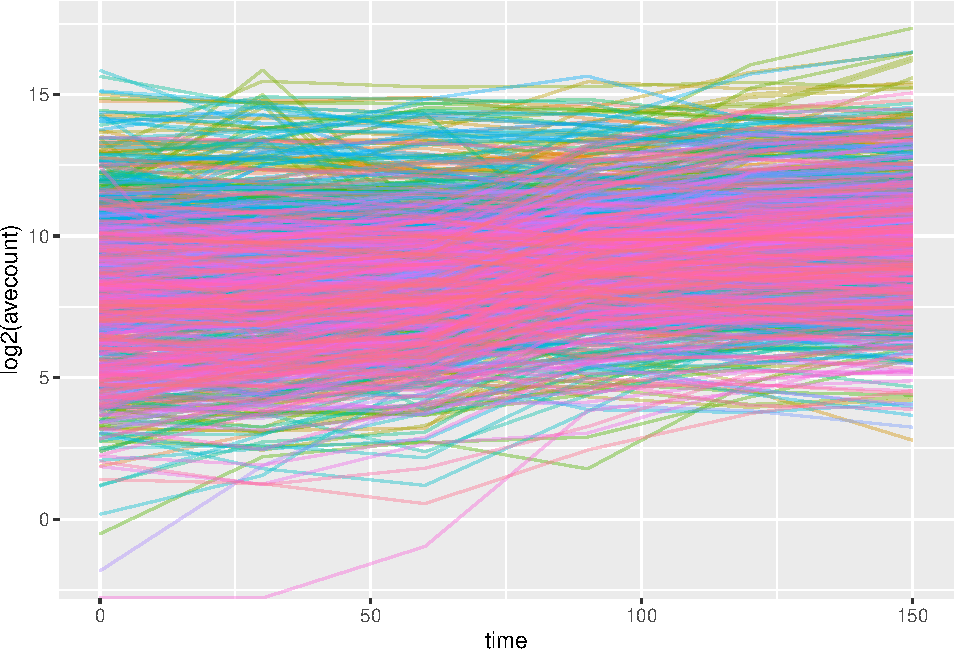
\includegraphics{EcoliTechnicalReport_files/figure-latex/plot DEGs-1.pdf}

In our case, these plots are not extremely helpful because they are so
overcrowded and it is difficult to see any trends. In Section 5, we will
jump into clustering methods and other analyses that can identify
specific gene profiles.

\subsubsection{\texorpdfstring{\textbf{4.3} Shiny
App}{4.3 Shiny App}}\label{shiny-app}

Shiny is an R package that allows us to create interactive web apps
inside of R. While our Shiny code is not interactive or compatible with
the HTML export format, this code runs within R and creates a pop-up app
that allows the viewer to visualize the gene expression data. Shiny is
especially helpful when trying to determine optimal cut-offs for
p-values or fold changes, or when switching between comparisons of the
same data.

\section{\texorpdfstring{\textbf{5}
Analysis}{5 Analysis}}\label{analysis}

\subsubsection{\texorpdfstring{\textbf{5.1} PAM
Clustering}{5.1 PAM Clustering}}\label{pam-clustering}

Partitioning Around Medoids (PAM) is a clustering method iteratively
groups genes into clusters of genes with similar profiles. For our code,
we input a dissimilarity matrix, which is the transposed matrix of the
correlation between each gene, based on their counts. We use the
transpose of the count matrix because we want all of the genes as
columns in order to calculate the correlation. To calculate correlation,
we specified the method as ``spearman'', however ``pearson'' returns
similar results. The PAM method determines clusters by:\\
\textbf{1.} choosing k center genes (medoids);\\
\textbf{2.} assigning all of the rest of the genes to the closest
medoids;\\
\textbf{3.} calculating new medoids from these clusters -- in our case,
this is based off of the dissimilarity matrix provided;\\
\textbf{4.} repeating steps 2 and 3 until the clusters and medoids stay
the same between iterations.

First, we compute the optimal k number of clusters. This package
\texttt{NbClust} runs through 30 different tests that each determine the
optimal k and plots the distribution of all 30 of the optimal k results
in order to determine the most common result and the \emph{most} optimal
k.

\begin{Shaded}
\begin{Highlighting}[]
\KeywordTok{rownames}\NormalTok{(EC_DEGs) <-}\StringTok{ }\NormalTok{EC_DEGs}\OperatorTok{$}\NormalTok{genename}
\NormalTok{EC_DEGs <-}\StringTok{ }\NormalTok{EC_DEGs }\OperatorTok
\StringTok{  }\NormalTok{dplyr}\OperatorTok{::}\KeywordTok{select}\NormalTok{(}\OperatorTok{-}\NormalTok{genename)}

\CommentTok{# Set `diss = NULL` because our data is not a dissimilarity matrix. }
\CommentTok{# We set `distance = euclidean` because euclidean distance is the distance measurement }
\CommentTok{# used by the kmeans method, which we specify as the method}
\NormalTok{k_test <-}\StringTok{ }\KeywordTok{NbClust}\NormalTok{(}\DataTypeTok{data =}\NormalTok{ EC_DEGs, }\DataTypeTok{diss =} \OtherTok{NULL}\NormalTok{, }\DataTypeTok{distance =} \StringTok{"euclidean"}\NormalTok{, }
                  \DataTypeTok{min.nc =} \DecValTok{2}\NormalTok{, }\DataTypeTok{max.nc =} \DecValTok{20}\NormalTok{, }\DataTypeTok{method =} \StringTok{"kmeans"}\NormalTok{)}
\end{Highlighting}
\end{Shaded}

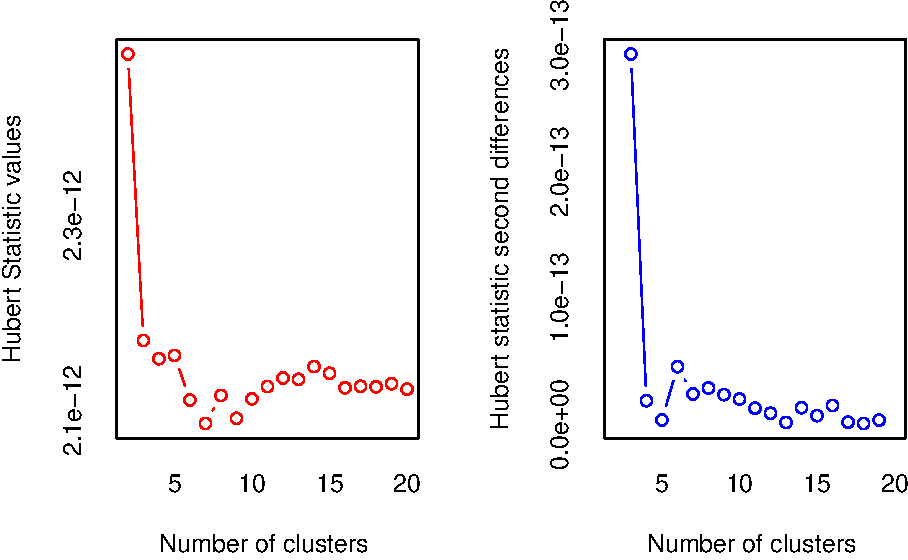
\includegraphics{EcoliTechnicalReport_files/figure-latex/calc optimal k-1.pdf}

\begin{verbatim}
## *** : The Hubert index is a graphical method of determining the number of clusters.
##                 In the plot of Hubert index, we seek a significant knee that corresponds to a 
##                 significant increase of the value of the measure i.e the significant peak in Hubert
##                 index second differences plot. 
## 
\end{verbatim}

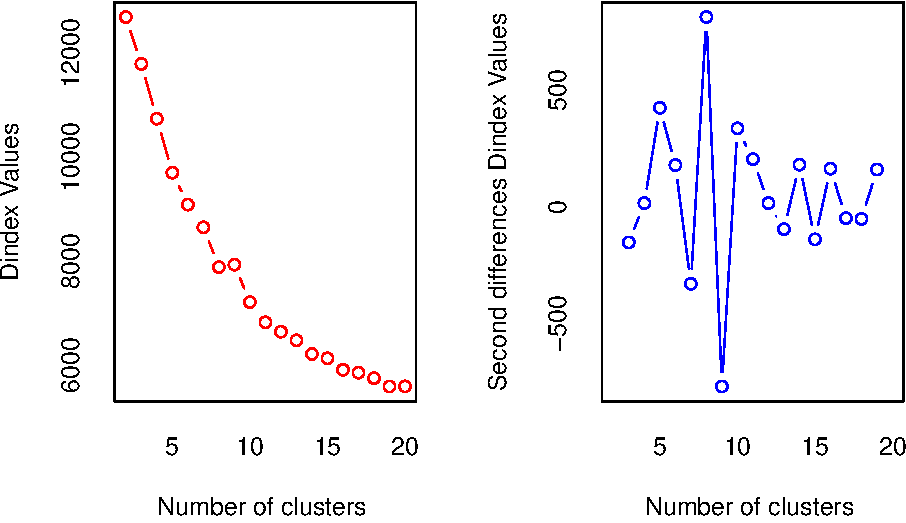
\includegraphics{EcoliTechnicalReport_files/figure-latex/calc optimal k-2.pdf}

\begin{verbatim}
## *** : The D index is a graphical method of determining the number of clusters. 
##                 In the plot of D index, we seek a significant knee (the significant peak in Dindex
##                 second differences plot) that corresponds to a significant increase of the value of
##                 the measure. 
##  
## ******************************************************************* 
## * Among all indices:                                                
## * 1 proposed 2 as the best number of clusters 
## * 13 proposed 3 as the best number of clusters 
## * 1 proposed 4 as the best number of clusters 
## * 3 proposed 16 as the best number of clusters 
## * 1 proposed 18 as the best number of clusters 
## * 1 proposed 19 as the best number of clusters 
## * 2 proposed 20 as the best number of clusters 
## 
##                    ***** Conclusion *****                            
##  
## * According to the majority rule, the best number of clusters is  3 
##  
##  
## *******************************************************************
\end{verbatim}

Take the results of this function with a grain of salt because it uses a
different clustering method than the PAM method we use. While this
program determines k = 3 to be the optimal number of clusters, we used k
= 6 so that we did not miss any unique profiles. {[}This is a potential
area for more research looking into the best k and the outcomes of the
clusters and the significance of their GO terms depending on the number
of clusters.{]} Then we use the PAM method to cluster the DEGs' count
data.

\begin{Shaded}
\begin{Highlighting}[]
\NormalTok{k =}\StringTok{ }\DecValTok{6}

\CommentTok{# Calculate the dissimilarity matrix}
\NormalTok{dissimilarity_matrix <-}\StringTok{ }\DecValTok{1} \OperatorTok{-}\StringTok{ }\KeywordTok{cor}\NormalTok{(}\KeywordTok{t}\NormalTok{(EC_DEGs), }\DataTypeTok{method =} \StringTok{"spearman"}\NormalTok{)}

\CommentTok{# Run the pam() function which clusters the data}
\CommentTok{# `pamonce = 3` speeds up the function by maximizing short cuts}
\NormalTok{EC_DESeq_clusters <-}\StringTok{ }\NormalTok{cluster}\OperatorTok{::}\KeywordTok{pam}\NormalTok{(}\DataTypeTok{x =}\NormalTok{ dissimilarity_matrix, }\DataTypeTok{k =}\NormalTok{ k, }\DataTypeTok{pamonce =} \DecValTok{3}\NormalTok{)}

\CommentTok{# Create a data table with the cluster name and genename}
\NormalTok{gene_cluster <-}\StringTok{ }\KeywordTok{data.frame}\NormalTok{(}\StringTok{"cluster"}\NormalTok{ =}\StringTok{ }\NormalTok{EC_DESeq_clusters}\OperatorTok{$}\NormalTok{clustering, }
                           \StringTok{"genename"}\NormalTok{ =}\StringTok{ }\KeywordTok{names}\NormalTok{(EC_DESeq_clusters}\OperatorTok{$}\NormalTok{clustering))}

\CommentTok{# Make a data frame with the names of the medoid for each of the k clusters}
\NormalTok{EC_PAM_medoids <-}\StringTok{ }\KeywordTok{data.frame}\NormalTok{(}\StringTok{"genename"}\NormalTok{ =}\StringTok{ }\KeywordTok{rownames}\NormalTok{(EC_DESeq_clusters}\OperatorTok{$}\NormalTok{medoids))}

\NormalTok{ec_norm_counts <-}\StringTok{ }\NormalTok{ec_normcounts }\OperatorTok
\StringTok{  }\KeywordTok{mutate}\NormalTok{(}\StringTok{"genename"}\NormalTok{ =}\StringTok{ }\KeywordTok{rownames}\NormalTok{(ec_normcounts))}

\CommentTok{# Join the normalized counts with the clusters of genes by their genename}
\NormalTok{EC_cluster_df <-}\StringTok{ }\KeywordTok{left_join}\NormalTok{(gene_cluster, ec_norm_counts, }\DataTypeTok{by =} \StringTok{"genename"}\NormalTok{)}
\end{Highlighting}
\end{Shaded}

Now, we will standardize our data using the \texttt{Mfuzz} package's
\texttt{standardise()} function. The function standardizes the data so
that each gene has a mean expression of 0 and a standard deviation of 1.
We standardize our data with the Fuzzy package in order to visualize and
understand the profiles within each cluster.

\begin{Shaded}
\begin{Highlighting}[]
\NormalTok{cluster_standard <-}\StringTok{ }\NormalTok{EC_cluster_df }\OperatorTok
\StringTok{  }\NormalTok{dplyr}\OperatorTok{::}\KeywordTok{select}\NormalTok{(}\OperatorTok{-}\NormalTok{cluster)}
\KeywordTok{rownames}\NormalTok{(cluster_standard) <-}\StringTok{ }\NormalTok{cluster_standard}\OperatorTok{$}\NormalTok{genename}
\NormalTok{cluster_standard <-}\StringTok{ }\NormalTok{cluster_standard }\OperatorTok
\StringTok{  }\NormalTok{dplyr}\OperatorTok{::}\KeywordTok{select}\NormalTok{(}\OperatorTok{-}\NormalTok{genename)}

\CommentTok{# Create a phenotype data frame, which describes the conditions/columns of the mnain data frame.}
\NormalTok{metadata <-}\StringTok{ }\KeywordTok{data.frame}\NormalTok{(}\DataTypeTok{labelDescription =} \KeywordTok{c}\NormalTok{(}\StringTok{"treat"}\NormalTok{, }\StringTok{"rep"}\NormalTok{, }\StringTok{"time"}\NormalTok{, }\StringTok{"timetreat"}\NormalTok{))}
\NormalTok{phenoData <-}\StringTok{ }\KeywordTok{new}\NormalTok{(}\StringTok{"AnnotatedDataFrame"}\NormalTok{, }\DataTypeTok{data=}\NormalTok{ec_coldata, }\DataTypeTok{varMetadata=}\NormalTok{metadata)}

\CommentTok{# Convert the gene expression data frame to a matrix}
\NormalTok{clusters <-}\StringTok{ }\KeywordTok{as.matrix}\NormalTok{(cluster_standard)}

\CommentTok{# Create an object of type `ExpressionSet`}
\NormalTok{eset <-}\StringTok{ }\NormalTok{Biobase}\OperatorTok{::}\KeywordTok{ExpressionSet}\NormalTok{(}\DataTypeTok{assayData =}\NormalTok{ clusters, }\DataTypeTok{phenoData =}\NormalTok{ phenoData)}

\CommentTok{# Plug `eset` into the `standardise()` function}
\CommentTok{# and extract the standardized matrix and convert it into a data frame}
\NormalTok{cluster_standardized <-}\StringTok{ }\NormalTok{Mfuzz}\OperatorTok{::}\KeywordTok{standardise}\NormalTok{(}\DataTypeTok{eset =}\NormalTok{ eset)}
\NormalTok{standard_clusters <-}\StringTok{ }\KeywordTok{data.frame}\NormalTok{(cluster_standardized}\OperatorTok{@}\NormalTok{assayData}\OperatorTok{$}\NormalTok{exprs)}
\NormalTok{standard_clusters}\OperatorTok{$}\NormalTok{genename <-}\StringTok{ }\KeywordTok{rownames}\NormalTok{(standard_clusters)}

\CommentTok{# Join the cluster data with the standardized expression counts}
\NormalTok{clusters <-}\StringTok{ }\KeywordTok{left_join}\NormalTok{(standard_clusters, gene_cluster, }\DataTypeTok{by =} \StringTok{"genename"}\NormalTok{)}
\end{Highlighting}
\end{Shaded}

Then, we can use the tidying pipeline (see Section 4.1 for more
information) to tidy the standardized data.

\begin{Shaded}
\begin{Highlighting}[]
\NormalTok{EC_counts_gath <-}\StringTok{ }\NormalTok{clusters }\OperatorTok
\StringTok{  }\KeywordTok{gather}\NormalTok{(}\OperatorTok{-}\KeywordTok{c}\NormalTok{(genename, cluster), }\DataTypeTok{key=}\StringTok{"sample"}\NormalTok{, }\DataTypeTok{value =} \StringTok{"rawcount"}\NormalTok{) }\OperatorTok
\StringTok{  }\KeywordTok{separate}\NormalTok{(sample, }\KeywordTok{c}\NormalTok{(}\StringTok{"treat"}\NormalTok{, }\StringTok{"rep_time"}\NormalTok{), }\StringTok{"_"}\NormalTok{) }\OperatorTok
\StringTok{  }\KeywordTok{mutate}\NormalTok{(}\DataTypeTok{rep =} \KeywordTok{ifelse}\NormalTok{(}\KeywordTok{substr}\NormalTok{(rep_time,}\DataTypeTok{start=}\DecValTok{1}\NormalTok{,}\DataTypeTok{stop =} \DecValTok{1}\NormalTok{) }\OperatorTok{==}\StringTok{ "A"}\NormalTok{, }\DecValTok{1}\NormalTok{, }
                        \KeywordTok{ifelse}\NormalTok{(}\KeywordTok{substr}\NormalTok{(rep_time,}\DataTypeTok{start=}\DecValTok{1}\NormalTok{,}\DataTypeTok{stop =} \DecValTok{1}\NormalTok{) }\OperatorTok{==}\StringTok{ "B"}\NormalTok{, }\DecValTok{2}\NormalTok{, }\DecValTok{3}\NormalTok{))) }\OperatorTok
\StringTok{  }\KeywordTok{mutate}\NormalTok{(}\DataTypeTok{time =} \KeywordTok{ifelse}\NormalTok{(}\KeywordTok{substr}\NormalTok{(rep_time,}\DataTypeTok{start=}\DecValTok{3}\NormalTok{,}\DataTypeTok{stop =} \DecValTok{3}\NormalTok{) }\OperatorTok{==}\StringTok{ "1"}\NormalTok{, }\DecValTok{0}\NormalTok{,}
                      \KeywordTok{ifelse}\NormalTok{(}\KeywordTok{substr}\NormalTok{(rep_time,}\DataTypeTok{start=}\DecValTok{3}\NormalTok{,}\DataTypeTok{stop =} \DecValTok{3}\NormalTok{) }\OperatorTok{==}\StringTok{ "2"}\NormalTok{, }\DecValTok{30}\NormalTok{,}
                             \KeywordTok{ifelse}\NormalTok{(}\KeywordTok{substr}\NormalTok{(rep_time,}\DataTypeTok{start=}\DecValTok{3}\NormalTok{,}\DataTypeTok{stop =} \DecValTok{3}\NormalTok{) }\OperatorTok{==}\StringTok{ "3"}\NormalTok{, }\DecValTok{60}\NormalTok{,}
                                    \KeywordTok{ifelse}\NormalTok{(}\KeywordTok{substr}\NormalTok{(rep_time,}\DataTypeTok{start=}\DecValTok{3}\NormalTok{,}\DataTypeTok{stop =} \DecValTok{3}\NormalTok{) }\OperatorTok{==}\StringTok{ "4"}\NormalTok{, }\DecValTok{90}\NormalTok{,}
                                           \KeywordTok{ifelse}\NormalTok{(}\KeywordTok{substr}\NormalTok{(rep_time,}\DataTypeTok{start=}\DecValTok{3}\NormalTok{,}\DataTypeTok{stop =} \DecValTok{3}\NormalTok{) }\OperatorTok{==}\StringTok{ "5"}\NormalTok{, }\DecValTok{120}\NormalTok{, }\DecValTok{150}\NormalTok{)))))) }\OperatorTok
\StringTok{  }\KeywordTok{mutate}\NormalTok{(}\DataTypeTok{treat =} \KeywordTok{ifelse}\NormalTok{(treat }\OperatorTok{==}\StringTok{ "JH01"}\NormalTok{, }\StringTok{"WT"}\NormalTok{,}\StringTok{"dRpoS"}\NormalTok{)) }\OperatorTok
\StringTok{  }\NormalTok{dplyr}\OperatorTok{::}\KeywordTok{select}\NormalTok{(}\OperatorTok{-}\KeywordTok{c}\NormalTok{(rep_time))}
                                      
\NormalTok{EC_counts_sum <-}\StringTok{ }\NormalTok{EC_counts_gath }\OperatorTok
\StringTok{  }\KeywordTok{group_by}\NormalTok{(genename, cluster, treat, time) }\OperatorTok
\StringTok{  }\NormalTok{dplyr}\OperatorTok{::}\KeywordTok{summarise}\NormalTok{(}\DataTypeTok{avecount =} \KeywordTok{mean}\NormalTok{(rawcount)) }\OperatorTok
\StringTok{  }\KeywordTok{filter}\NormalTok{(treat }\OperatorTok{==}\StringTok{ "WT"}\NormalTok{) }\OperatorTok
\StringTok{  }\KeywordTok{filter}\NormalTok{(}\OperatorTok{!}\KeywordTok{is.na}\NormalTok{(cluster))}
\KeywordTok{colnames}\NormalTok{(EC_counts_sum) <-}\StringTok{ }\KeywordTok{c}\NormalTok{(}\StringTok{"genename"}\NormalTok{, }\StringTok{"cluster"}\NormalTok{, }\StringTok{"treat"}\NormalTok{, }\StringTok{"time"}\NormalTok{, }\StringTok{"avecount"}\NormalTok{)}
\end{Highlighting}
\end{Shaded}

Next, we extract the medoid genes and tidy the medoid gene expression
data in order to plot the medoids on top of the gene clusters.

\begin{Shaded}
\begin{Highlighting}[]
\CommentTok{# Create a data frame that joins the medoid gene names}
\CommentTok{# and their standardized expression values}
\NormalTok{EC_medoid_df <-}\StringTok{ }\KeywordTok{left_join}\NormalTok{(EC_PAM_medoids, clusters, }\DataTypeTok{by =} \StringTok{"genename"}\NormalTok{) }\OperatorTok
\StringTok{  }\NormalTok{dplyr}\OperatorTok{::}\KeywordTok{select}\NormalTok{(}\OperatorTok{-}\NormalTok{cluster) }\OperatorTok
\StringTok{  }\KeywordTok{mutate}\NormalTok{(}\DataTypeTok{cluster =} \KeywordTok{c}\NormalTok{(}\DecValTok{1}\OperatorTok{:}\NormalTok{k))}

\CommentTok{# Tidy medoid data (pipeline detailed in section 4.1)}
\NormalTok{EC_counts_gath_med <-}\StringTok{ }\NormalTok{EC_medoid_df }\OperatorTok
\StringTok{  }\KeywordTok{gather}\NormalTok{(}\OperatorTok{-}\KeywordTok{c}\NormalTok{(genename, cluster), }\DataTypeTok{key=}\StringTok{"sample"}\NormalTok{, }\DataTypeTok{value =} \StringTok{"rawcount"}\NormalTok{) }\OperatorTok
\StringTok{  }\KeywordTok{separate}\NormalTok{(sample, }\KeywordTok{c}\NormalTok{(}\StringTok{"treat"}\NormalTok{, }\StringTok{"rep_time"}\NormalTok{), }\StringTok{"_"}\NormalTok{) }\OperatorTok
\StringTok{  }\KeywordTok{mutate}\NormalTok{(}\DataTypeTok{rep =} \KeywordTok{ifelse}\NormalTok{(}\KeywordTok{substr}\NormalTok{(rep_time,}\DataTypeTok{start=}\DecValTok{1}\NormalTok{,}\DataTypeTok{stop =} \DecValTok{1}\NormalTok{) }\OperatorTok{==}\StringTok{ "A"}\NormalTok{, }\DecValTok{1}\NormalTok{, }
                        \KeywordTok{ifelse}\NormalTok{(}\KeywordTok{substr}\NormalTok{(rep_time,}\DataTypeTok{start=}\DecValTok{1}\NormalTok{,}\DataTypeTok{stop =} \DecValTok{1}\NormalTok{) }\OperatorTok{==}\StringTok{ "B"}\NormalTok{, }\DecValTok{2}\NormalTok{, }\DecValTok{3}\NormalTok{))) }\OperatorTok
\StringTok{  }\KeywordTok{mutate}\NormalTok{(}\DataTypeTok{time =} \KeywordTok{ifelse}\NormalTok{(}\KeywordTok{substr}\NormalTok{(rep_time,}\DataTypeTok{start=}\DecValTok{3}\NormalTok{,}\DataTypeTok{stop =} \DecValTok{3}\NormalTok{) }\OperatorTok{==}\StringTok{ "1"}\NormalTok{, }\DecValTok{0}\NormalTok{,}
                      \KeywordTok{ifelse}\NormalTok{(}\KeywordTok{substr}\NormalTok{(rep_time,}\DataTypeTok{start=}\DecValTok{3}\NormalTok{,}\DataTypeTok{stop =} \DecValTok{3}\NormalTok{) }\OperatorTok{==}\StringTok{ "2"}\NormalTok{, }\DecValTok{30}\NormalTok{,}
                             \KeywordTok{ifelse}\NormalTok{(}\KeywordTok{substr}\NormalTok{(rep_time,}\DataTypeTok{start=}\DecValTok{3}\NormalTok{,}\DataTypeTok{stop =} \DecValTok{3}\NormalTok{) }\OperatorTok{==}\StringTok{ "3"}\NormalTok{, }\DecValTok{60}\NormalTok{,}
                                    \KeywordTok{ifelse}\NormalTok{(}\KeywordTok{substr}\NormalTok{(rep_time,}\DataTypeTok{start=}\DecValTok{3}\NormalTok{,}\DataTypeTok{stop =} \DecValTok{3}\NormalTok{) }\OperatorTok{==}\StringTok{ "4"}\NormalTok{, }\DecValTok{90}\NormalTok{,}
                                           \KeywordTok{ifelse}\NormalTok{(}\KeywordTok{substr}\NormalTok{(rep_time,}\DataTypeTok{start=}\DecValTok{3}\NormalTok{,}\DataTypeTok{stop =} \DecValTok{3}\NormalTok{) }\OperatorTok{==}\StringTok{ "5"}\NormalTok{, }\DecValTok{120}\NormalTok{, }\DecValTok{150}\NormalTok{)))))) }\OperatorTok
\StringTok{  }\KeywordTok{mutate}\NormalTok{(}\DataTypeTok{treat =} \KeywordTok{ifelse}\NormalTok{(treat }\OperatorTok{==}\StringTok{ "JH01"}\NormalTok{, }\StringTok{"WT"}\NormalTok{,}\StringTok{"dRpoS"}\NormalTok{)) }\OperatorTok
\StringTok{  }\NormalTok{dplyr}\OperatorTok{::}\KeywordTok{select}\NormalTok{(}\OperatorTok{-}\KeywordTok{c}\NormalTok{(rep_time))}
                                      
\NormalTok{EC_counts_sum_med <-}\StringTok{ }\NormalTok{EC_counts_gath_med }\OperatorTok
\StringTok{  }\KeywordTok{group_by}\NormalTok{(genename, cluster, treat, time) }\OperatorTok
\StringTok{  }\NormalTok{dplyr}\OperatorTok{::}\KeywordTok{summarise}\NormalTok{(}\DataTypeTok{avecount =} \KeywordTok{mean}\NormalTok{(rawcount)) }\OperatorTok
\StringTok{  }\KeywordTok{filter}\NormalTok{(treat }\OperatorTok{==}\StringTok{ "WT"}\NormalTok{)}
\KeywordTok{colnames}\NormalTok{(EC_counts_sum_med) <-}\StringTok{ }\KeywordTok{c}\NormalTok{(}\StringTok{"genename"}\NormalTok{, }\StringTok{"cluster"}\NormalTok{, }\StringTok{"treat"}\NormalTok{, }\StringTok{"time"}\NormalTok{, }\StringTok{"avecount"}\NormalTok{)}
\end{Highlighting}
\end{Shaded}

Now we can plot our clusters using \texttt{ggplot}.

\begin{Shaded}
\begin{Highlighting}[]
\NormalTok{EC_counts_sum }\OperatorTok
\StringTok{  }\CommentTok{#Because we have standardized our data using the `Mfuzz` package,}
\StringTok{  }\CommentTok{# we do not need to  transform the y-axis - just use `avecount`}
\StringTok{  }\KeywordTok{ggplot}\NormalTok{(}\KeywordTok{aes}\NormalTok{(}\DataTypeTok{x=}\NormalTok{time, }\DataTypeTok{y=}\NormalTok{avecount)) }\OperatorTok{+}
\StringTok{  }\CommentTok{# We set `group = genename` and `color = as.factor(cluster)` }
\StringTok{  }\CommentTok{# in order to keep each gene separated and color by cluster. }
\StringTok{  }\CommentTok{# set alpha to a decimal smaller than 1 in order to see the overlap of genes within each cluster.}
\StringTok{  }\KeywordTok{geom_line}\NormalTok{(}\KeywordTok{aes}\NormalTok{(}\DataTypeTok{group =}\NormalTok{ genename, }\DataTypeTok{color =} \KeywordTok{as.factor}\NormalTok{(cluster)), }
            \DataTypeTok{lineend =} \StringTok{"round"}\NormalTok{ , }\DataTypeTok{alpha =} \FloatTok{0.3}\NormalTok{) }\OperatorTok{+}
\StringTok{  }\CommentTok{# We use `facet_wrap()` to separate the clusters into different plots, }
\StringTok{  }\CommentTok{# with the same scale}
\StringTok{  }\KeywordTok{facet_wrap}\NormalTok{(}\OperatorTok{~}\KeywordTok{factor}\NormalTok{(cluster, }\DataTypeTok{labels =} \KeywordTok{c}\NormalTok{(}\StringTok{"Cluster 1"}\NormalTok{, }\StringTok{"Cluster 2"}\NormalTok{, }
                                         \StringTok{"Cluster 3"}\NormalTok{, }\StringTok{"Cluster 4"}\NormalTok{, }
                                         \StringTok{"Cluster 5"}\NormalTok{, }\StringTok{"Cluster 6"}\NormalTok{))) }\OperatorTok{+}
\StringTok{  }\CommentTok{# Plot the medoids on top of each cluster.}
\StringTok{  }\KeywordTok{geom_line}\NormalTok{(}\DataTypeTok{data =}\NormalTok{ EC_counts_sum_med, }\KeywordTok{aes}\NormalTok{(}\DataTypeTok{x=}\NormalTok{time, }\DataTypeTok{y=}\NormalTok{avecount, }\DataTypeTok{group =}\NormalTok{ genename), }\DataTypeTok{size =} \DecValTok{1}\NormalTok{) }\OperatorTok{+}
\StringTok{  }\KeywordTok{theme}\NormalTok{(}\DataTypeTok{legend.position =} \StringTok{"none"}\NormalTok{, }\DataTypeTok{panel.background =} \KeywordTok{element_blank}\NormalTok{(), }
        \DataTypeTok{strip.text =} \KeywordTok{element_text}\NormalTok{(}\DataTypeTok{size =} \DecValTok{20}\NormalTok{), }
        \DataTypeTok{axis.title =} \KeywordTok{element_text}\NormalTok{(}\DataTypeTok{size =} \DecValTok{13}\NormalTok{), }\DataTypeTok{axis.text =} \KeywordTok{element_text}\NormalTok{(}\DataTypeTok{size =} \DecValTok{10}\NormalTok{))}
\end{Highlighting}
\end{Shaded}

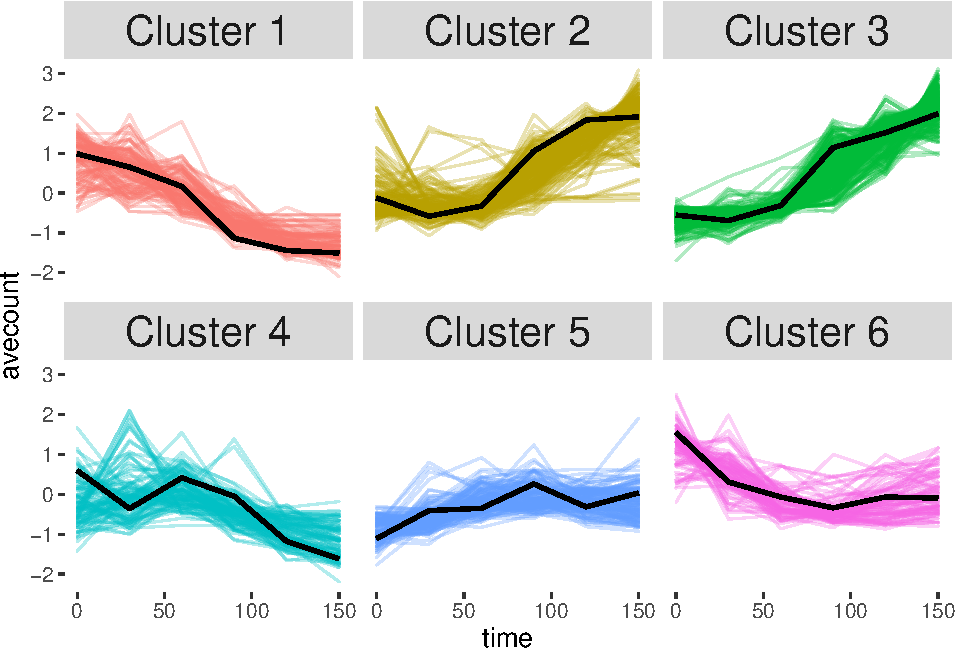
\includegraphics{EcoliTechnicalReport_files/figure-latex/plot clusters-1.pdf}

And we create a list of data frames that contain each clusters list of
genes.

\begin{Shaded}
\begin{Highlighting}[]
\NormalTok{cluster_genes <-}\StringTok{ }\KeywordTok{data.frame}\NormalTok{(}\StringTok{"genename"}\NormalTok{ =}\StringTok{ }\NormalTok{gene_cluster}\OperatorTok{$}\NormalTok{genename)}
\KeywordTok{rownames}\NormalTok{(cluster_genes) <-}\StringTok{ }\NormalTok{cluster_genes}\OperatorTok{$}\NormalTok{genename}
\NormalTok{cluster_genes <-}\StringTok{ }\KeywordTok{left_join}\NormalTok{(cluster_genes, gene_cluster, }\DataTypeTok{by =} \StringTok{"genename"}\NormalTok{) }\OperatorTok
\StringTok{  }\KeywordTok{filter}\NormalTok{(}\OperatorTok{!}\KeywordTok{is.na}\NormalTok{(genename))}
\KeywordTok{rownames}\NormalTok{(cluster_genes) <-}\StringTok{ }\NormalTok{cluster_genes}\OperatorTok{$}\NormalTok{genename}

\CommentTok{# List of data frames with gene names for each cluster called `EC_cluster`}
\NormalTok{EC_cluster <-}\StringTok{ }\KeywordTok{c}\NormalTok{()}
\NormalTok{EC_cluster}\OperatorTok{$}\NormalTok{cluster1 <-}\StringTok{ }\NormalTok{cluster_genes }\OperatorTok
\StringTok{  }\KeywordTok{filter}\NormalTok{(cluster }\OperatorTok{==}\StringTok{ }\DecValTok{1}\NormalTok{) }\OperatorTok
\StringTok{  }\NormalTok{dplyr}\OperatorTok{::}\KeywordTok{select}\NormalTok{(genename)}
\NormalTok{EC_cluster}\OperatorTok{$}\NormalTok{cluster2 <-}\StringTok{ }\NormalTok{cluster_genes }\OperatorTok
\StringTok{  }\KeywordTok{filter}\NormalTok{(cluster }\OperatorTok{==}\StringTok{ }\DecValTok{2}\NormalTok{) }\OperatorTok
\StringTok{  }\NormalTok{dplyr}\OperatorTok{::}\KeywordTok{select}\NormalTok{(genename)}
\NormalTok{EC_cluster}\OperatorTok{$}\NormalTok{cluster3 <-}\StringTok{ }\NormalTok{cluster_genes }\OperatorTok
\StringTok{  }\KeywordTok{filter}\NormalTok{(cluster }\OperatorTok{==}\StringTok{ }\DecValTok{3}\NormalTok{) }\OperatorTok
\StringTok{  }\NormalTok{dplyr}\OperatorTok{::}\KeywordTok{select}\NormalTok{(genename)}
\NormalTok{EC_cluster}\OperatorTok{$}\NormalTok{cluster4 <-}\StringTok{ }\NormalTok{cluster_genes }\OperatorTok
\StringTok{  }\KeywordTok{filter}\NormalTok{(cluster }\OperatorTok{==}\StringTok{ }\DecValTok{4}\NormalTok{) }\OperatorTok
\StringTok{  }\NormalTok{dplyr}\OperatorTok{::}\KeywordTok{select}\NormalTok{(genename)}
\NormalTok{EC_cluster}\OperatorTok{$}\NormalTok{cluster5 <-}\StringTok{ }\NormalTok{cluster_genes }\OperatorTok
\StringTok{  }\KeywordTok{filter}\NormalTok{(cluster }\OperatorTok{==}\StringTok{ }\DecValTok{5}\NormalTok{) }\OperatorTok
\StringTok{  }\NormalTok{dplyr}\OperatorTok{::}\KeywordTok{select}\NormalTok{(genename)}
\NormalTok{EC_cluster}\OperatorTok{$}\NormalTok{cluster6 <-}\StringTok{ }\NormalTok{cluster_genes }\OperatorTok
\StringTok{  }\KeywordTok{filter}\NormalTok{(cluster }\OperatorTok{==}\StringTok{ }\DecValTok{6}\NormalTok{) }\OperatorTok
\StringTok{  }\NormalTok{dplyr}\OperatorTok{::}\KeywordTok{select}\NormalTok{(genename)}
\end{Highlighting}
\end{Shaded}

\subsubsection{\texorpdfstring{\textbf{5.2} Gene Ontology
Analysis}{5.2 Gene Ontology Analysis}}\label{gene-ontology-analysis}

Gene Ontology (GO) analysis is a tool used in order to determine whether
specified groups of genes have unique biological significance. Gene
Ontology Analysis relies on a list of GO terms, which is a list of all
of the genetic functions within the organism and the respective genes
involved in each of those functions (Alexa and Rahnenfuhrer, 2019). For
each of the specified groups of genes, the analysis determines whether
the list of genes is disproportionately distributed across genetic
functions. Compared to the null (uniform) distribution of the group's
genes across all genetic functions, are the group's genes significantly
enriched within specific functions?

To answer this question, we use a package called \texttt{TopGO} which
has a database with all of \emph{E. coli}'s GO terms. We can specify the
statistical method used to determine whether a GO term is significant
within a group of genes. Below, I provide code for the Fisher method,
but the other option, a Kolmogorov-Smirnov test, is a simple
substitution. GO terms are classified within three different categories:
Biological Processes, Molecular Functions, and Cellular Components.
After consultation with Professor Stoebel, Biological Process appears to
be the most relevant in this research. However, the other two types have
positives that could be more useful in other work: Molecular Function
can offer specific, molecular-level information and Cellular Component
can provide broad information about cell parts and structure.

\begin{Shaded}
\begin{Highlighting}[]
\CommentTok{# Create a function that runs GO analysis, }
\CommentTok{# with the two parameters being the type of GO and the cluster number.}
\NormalTok{go_enrich <-}\StringTok{ }\ControlFlowTok{function}\NormalTok{(go_type, k) \{}
  \CommentTok{# Create a function within the function that }
  \CommentTok{# returns a logical list marking whether or not a gene is in cluster k}
\NormalTok{  selection <-}\StringTok{ }\ControlFlowTok{function}\NormalTok{(k) \{}
\NormalTok{    gene_clust <-}\StringTok{ }\NormalTok{cluster_genes}\OperatorTok{$}\NormalTok{cluster }\OperatorTok{==}\StringTok{ }\NormalTok{k}
    \KeywordTok{return}\NormalTok{(gene_clust)}
\NormalTok{  \}}
  \CommentTok{# Create a factor with 2 levels: }
  \CommentTok{# (1) integer versions (TRUE = 1 and FALSE = 0) of the logical result }
  \CommentTok{# from the above `selection()` function }
  \CommentTok{# and (2) their respective gene name}
\NormalTok{  GeneList <-}\StringTok{ }\KeywordTok{factor}\NormalTok{(}\KeywordTok{as.integer}\NormalTok{(}\KeywordTok{selection}\NormalTok{(k)))}
  \KeywordTok{names}\NormalTok{(GeneList) <-}\StringTok{ }\NormalTok{cluster_genes}\OperatorTok{$}\NormalTok{genename}
  
  \CommentTok{# Map gene IDs to GO terms, both from database. }
  \CommentTok{# Set `whichOnto = go_type` so that the function specifies the type of GO terms }
  \CommentTok{# and set `ID = "symbol"` because our gene data is identified }
  \CommentTok{# by their symbol, the four letter combination associated with each gene}
\NormalTok{  annot <-}\StringTok{ }\KeywordTok{annFUN.org}\NormalTok{(}\DataTypeTok{whichOnto =}\NormalTok{ go_type, }
                      \DataTypeTok{feasibleGenes =} \OtherTok{NULL}\NormalTok{, }\DataTypeTok{mapping =} \StringTok{"org.EcK12.eg"}\NormalTok{, }\DataTypeTok{ID =} \StringTok{"symbol"}\NormalTok{)}
  
  \CommentTok{# Create a `topGOdata` object. Again, specify `ontology = go_type`. }
  \CommentTok{# Set `allGenes = GeneList` which is our factor object with 1s and 0s and gene names. }
  \CommentTok{# Then we set `annot = annFUN.GO2genes` and `GO2genes = annot`, }
  \CommentTok{# our previous object of mapped gene IDs and their GO terms.}
\NormalTok{  GOdata <-}\StringTok{ }\KeywordTok{new}\NormalTok{(}\StringTok{"topGOdata"}\NormalTok{, }\DataTypeTok{ontology=}\NormalTok{go_type, }\DataTypeTok{allGenes=}\NormalTok{GeneList,}
                \DataTypeTok{annot=}\NormalTok{annFUN.GO2genes, }\DataTypeTok{GO2genes =}\NormalTok{ annot, }
                \DataTypeTok{geneSelectionFun =}\NormalTok{ selection, }\DataTypeTok{nodeSize =} \DecValTok{5}\NormalTok{)}
  
  \CommentTok{# Run the GO analysis, specifying the algorithm and statistic. }
  \CommentTok{# If a Kolmogorov-Smirnov test is preferred, }
  \CommentTok{# change `statistic = "fisher"` to `statistic = "ks"` and rename object as `resultKS`.}
\NormalTok{  resultFis <-}\StringTok{ }\KeywordTok{runTest}\NormalTok{(GOdata, }\DataTypeTok{algorithm =} \StringTok{"classic"}\NormalTok{, }\DataTypeTok{statistic =} \StringTok{"fisher"}\NormalTok{)}
  
  \CommentTok{# Generate a table with the results ranked by their p-value. }
  \CommentTok{# If a Kolmogorov-Smirnov test is preferred, }
  \CommentTok{# change `fisherPval = "resultFis"` to `ksPval = "resultKS"`}
\NormalTok{  goEnrich <-}\StringTok{ }\KeywordTok{GenTable}\NormalTok{(GOdata, }\DataTypeTok{fisherPval =}\NormalTok{ resultFis, }\DataTypeTok{topNodes =} \DecValTok{30}\NormalTok{)}
  
  \CommentTok{# Create a column that identifies the genes from the cluster }
  \CommentTok{# within each GO term. Mostly NULL values}
\NormalTok{  ind <-}\StringTok{ }\KeywordTok{match}\NormalTok{(goEnrich}\OperatorTok{$}\NormalTok{GO.ID, }\KeywordTok{names}\NormalTok{(annot))}
\NormalTok{  goEnrich}\OperatorTok{$}\NormalTok{Gene <-}\StringTok{ }\NormalTok{annot[ind]}
  \KeywordTok{return}\NormalTok{(goEnrich)}
\NormalTok{\}}

\CommentTok{# Run the `go_enrich` function for each type within each cluster }
\CommentTok{# and bind the results, specifying the type of GO term in each case}
\NormalTok{bp <-}\StringTok{ }\KeywordTok{go_enrich}\NormalTok{(}\StringTok{"BP"}\NormalTok{, }\DecValTok{1}\NormalTok{) }\OperatorTok
\StringTok{  }\KeywordTok{mutate}\NormalTok{(}\StringTok{"Type"}\NormalTok{ =}\StringTok{ "Biological Process"}\NormalTok{)}
\NormalTok{mf <-}\StringTok{ }\KeywordTok{go_enrich}\NormalTok{(}\StringTok{"MF"}\NormalTok{, }\DecValTok{1}\NormalTok{) }\OperatorTok
\StringTok{  }\KeywordTok{mutate}\NormalTok{(}\StringTok{"Type"}\NormalTok{ =}\StringTok{ "Molecular Function"}\NormalTok{)}
\NormalTok{cc <-}\StringTok{ }\KeywordTok{go_enrich}\NormalTok{(}\StringTok{"CC"}\NormalTok{, }\DecValTok{1}\NormalTok{) }\OperatorTok
\StringTok{  }\KeywordTok{mutate}\NormalTok{(}\StringTok{"Type"}\NormalTok{ =}\StringTok{ "Cellular Component"}\NormalTok{)}
\NormalTok{cluster1_genes <-}\StringTok{ }\KeywordTok{bind_rows}\NormalTok{(bp, mf, cc)}

\NormalTok{bp <-}\StringTok{ }\KeywordTok{go_enrich}\NormalTok{(}\StringTok{"BP"}\NormalTok{, }\DecValTok{2}\NormalTok{) }\OperatorTok
\StringTok{  }\KeywordTok{mutate}\NormalTok{(}\StringTok{"Type"}\NormalTok{ =}\StringTok{ "Biological Process"}\NormalTok{)}
\NormalTok{mf <-}\StringTok{ }\KeywordTok{go_enrich}\NormalTok{(}\StringTok{"MF"}\NormalTok{, }\DecValTok{2}\NormalTok{) }\OperatorTok
\StringTok{  }\KeywordTok{mutate}\NormalTok{(}\StringTok{"Type"}\NormalTok{ =}\StringTok{ "Molecular Function"}\NormalTok{)}
\NormalTok{cc <-}\StringTok{ }\KeywordTok{go_enrich}\NormalTok{(}\StringTok{"CC"}\NormalTok{, }\DecValTok{2}\NormalTok{) }\OperatorTok
\StringTok{  }\KeywordTok{mutate}\NormalTok{(}\StringTok{"Type"}\NormalTok{ =}\StringTok{ "Cellular Component"}\NormalTok{)}
\NormalTok{cluster2_genes <-}\StringTok{ }\KeywordTok{bind_rows}\NormalTok{(bp, mf, cc)}

\NormalTok{bp <-}\StringTok{ }\KeywordTok{go_enrich}\NormalTok{(}\StringTok{"BP"}\NormalTok{, }\DecValTok{3}\NormalTok{) }\OperatorTok
\StringTok{  }\KeywordTok{mutate}\NormalTok{(}\StringTok{"Type"}\NormalTok{ =}\StringTok{ "Biological Process"}\NormalTok{)}
\NormalTok{mf <-}\StringTok{ }\KeywordTok{go_enrich}\NormalTok{(}\StringTok{"MF"}\NormalTok{, }\DecValTok{3}\NormalTok{) }\OperatorTok
\StringTok{  }\KeywordTok{mutate}\NormalTok{(}\StringTok{"Type"}\NormalTok{ =}\StringTok{ "Molecular Function"}\NormalTok{)}
\NormalTok{cc <-}\StringTok{ }\KeywordTok{go_enrich}\NormalTok{(}\StringTok{"CC"}\NormalTok{, }\DecValTok{3}\NormalTok{) }\OperatorTok
\StringTok{  }\KeywordTok{mutate}\NormalTok{(}\StringTok{"Type"}\NormalTok{ =}\StringTok{ "Cellular Component"}\NormalTok{)}
\NormalTok{cluster3_genes <-}\StringTok{ }\KeywordTok{bind_rows}\NormalTok{(bp, mf, cc)}

\NormalTok{bp <-}\StringTok{ }\KeywordTok{go_enrich}\NormalTok{(}\StringTok{"BP"}\NormalTok{, }\DecValTok{4}\NormalTok{) }\OperatorTok
\StringTok{  }\KeywordTok{mutate}\NormalTok{(}\StringTok{"Type"}\NormalTok{ =}\StringTok{ "Biological Process"}\NormalTok{)}
\NormalTok{mf <-}\StringTok{ }\KeywordTok{go_enrich}\NormalTok{(}\StringTok{"MF"}\NormalTok{, }\DecValTok{4}\NormalTok{) }\OperatorTok
\StringTok{  }\KeywordTok{mutate}\NormalTok{(}\StringTok{"Type"}\NormalTok{ =}\StringTok{ "Molecular Function"}\NormalTok{)}
\NormalTok{cc <-}\StringTok{ }\KeywordTok{go_enrich}\NormalTok{(}\StringTok{"CC"}\NormalTok{, }\DecValTok{4}\NormalTok{) }\OperatorTok
\StringTok{  }\KeywordTok{mutate}\NormalTok{(}\StringTok{"Type"}\NormalTok{ =}\StringTok{ "Cellular Component"}\NormalTok{)}
\NormalTok{cluster4_genes <-}\StringTok{ }\KeywordTok{bind_rows}\NormalTok{(bp, mf, cc)}

\NormalTok{bp <-}\StringTok{ }\KeywordTok{go_enrich}\NormalTok{(}\StringTok{"BP"}\NormalTok{, }\DecValTok{5}\NormalTok{) }\OperatorTok
\StringTok{  }\KeywordTok{mutate}\NormalTok{(}\StringTok{"Type"}\NormalTok{ =}\StringTok{ "Biological Process"}\NormalTok{)}
\NormalTok{mf <-}\StringTok{ }\KeywordTok{go_enrich}\NormalTok{(}\StringTok{"MF"}\NormalTok{, }\DecValTok{5}\NormalTok{) }\OperatorTok
\StringTok{  }\KeywordTok{mutate}\NormalTok{(}\StringTok{"Type"}\NormalTok{ =}\StringTok{ "Molecular Function"}\NormalTok{)}
\NormalTok{cc <-}\StringTok{ }\KeywordTok{go_enrich}\NormalTok{(}\StringTok{"CC"}\NormalTok{, }\DecValTok{5}\NormalTok{) }\OperatorTok
\StringTok{  }\KeywordTok{mutate}\NormalTok{(}\StringTok{"Type"}\NormalTok{ =}\StringTok{ "Cellular Component"}\NormalTok{)}
\NormalTok{cluster5_genes <-}\StringTok{ }\KeywordTok{bind_rows}\NormalTok{(bp, mf, cc)}

\NormalTok{bp <-}\StringTok{ }\KeywordTok{go_enrich}\NormalTok{(}\StringTok{"BP"}\NormalTok{, }\DecValTok{6}\NormalTok{) }\OperatorTok
\StringTok{  }\KeywordTok{mutate}\NormalTok{(}\StringTok{"Type"}\NormalTok{ =}\StringTok{ "Biological Process"}\NormalTok{)}
\NormalTok{mf <-}\StringTok{ }\KeywordTok{go_enrich}\NormalTok{(}\StringTok{"MF"}\NormalTok{, }\DecValTok{6}\NormalTok{) }\OperatorTok
\StringTok{  }\KeywordTok{mutate}\NormalTok{(}\StringTok{"Type"}\NormalTok{ =}\StringTok{ "Molecular Function"}\NormalTok{)}
\NormalTok{cc <-}\StringTok{ }\KeywordTok{go_enrich}\NormalTok{(}\StringTok{"CC"}\NormalTok{, }\DecValTok{6}\NormalTok{) }\OperatorTok
\StringTok{  }\KeywordTok{mutate}\NormalTok{(}\StringTok{"Type"}\NormalTok{ =}\StringTok{ "Cellular Component"}\NormalTok{)}
\NormalTok{cluster6_genes <-}\StringTok{ }\KeywordTok{bind_rows}\NormalTok{(bp, mf, cc)}

\CommentTok{# Create a list of data frames with the results from each of the clusters}
\NormalTok{GO_clusters <-}\StringTok{ }\KeywordTok{c}\NormalTok{()}
\NormalTok{GO_clusters}\OperatorTok{$}\NormalTok{cl1 <-}\StringTok{ }\NormalTok{cluster1_genes}
\NormalTok{GO_clusters}\OperatorTok{$}\NormalTok{cl2 <-}\StringTok{ }\NormalTok{cluster2_genes}
\NormalTok{GO_clusters}\OperatorTok{$}\NormalTok{cl3 <-}\StringTok{ }\NormalTok{cluster3_genes}
\NormalTok{GO_clusters}\OperatorTok{$}\NormalTok{cl4 <-}\StringTok{ }\NormalTok{cluster4_genes}
\NormalTok{GO_clusters}\OperatorTok{$}\NormalTok{cl5 <-}\StringTok{ }\NormalTok{cluster5_genes}
\NormalTok{GO_clusters}\OperatorTok{$}\NormalTok{cl6 <-}\StringTok{ }\NormalTok{cluster6_genes}
\end{Highlighting}
\end{Shaded}

\subsubsection{\texorpdfstring{\textbf{5.3} Gene Set Enrichment
Analysis}{5.3 Gene Set Enrichment Analysis}}\label{gene-set-enrichment-analysis}

Gene Set Enrichment Analysis (GSEA) is a tool that allows us to test
whether or not a determined set of genes is enriched in a list of genes
with different levels of differential expression, noted by a test
statistic. GSEA requires this list of genes to have a ranking statistic.
In our case, we used a p-value statistic which describes the
significance of the gene's differential expression. GSEA results with
high positive enrichment scores indicate enrichment at the top of the
ranked gene list, while large negative enrichment scores indicate
enrichment at the bottom of the list.

We compared each the 6 clusters to the lists of sensitive, insensitive,
and linear genes to determine whether the sensitive, insensitive, or
linear genes were enriched in any of our clusters. That is, for example,
were there more sensitive genes in cluster 1 than would be expected
under a uniform distribution of sensitive genes? Our results were not
very significant, however further analysis could potentially check other
gene sets for enrichment.

\begin{Shaded}
\begin{Highlighting}[]
\CommentTok{# create data frame for ranked list with all genenames and pvalues}
\CommentTok{# I used the gene list output by DESeq2 because this list has}
\CommentTok{# an adjusted pvalue associated with each gene}
\CommentTok{# and seemed to capture a lot of the genes from the venn diagram}
\NormalTok{ec_Stat <-}\StringTok{ }\KeywordTok{data.frame}\NormalTok{(}\StringTok{"genename"}\NormalTok{ =}\StringTok{ }\NormalTok{resSig}\OperatorTok{$}\NormalTok{genename, }\StringTok{"padj"}\NormalTok{ =}\StringTok{ }\NormalTok{resSig}\OperatorTok{$}\NormalTok{padj)}

\NormalTok{stat_all <-}\StringTok{ }\NormalTok{ec_Stat}\OperatorTok{$}\NormalTok{padj}
\KeywordTok{names}\NormalTok{(stat_all) <-}\StringTok{ }\NormalTok{ec_Stat}\OperatorTok{$}\NormalTok{genename}
  
\NormalTok{cluster1 <-}\StringTok{ }\KeywordTok{left_join}\NormalTok{(EC_cluster}\OperatorTok{$}\NormalTok{cluster1,ec_Stat, }\DataTypeTok{by =} \StringTok{"genename"}\NormalTok{) }\OperatorTok
\StringTok{  }\KeywordTok{filter}\NormalTok{(}\OperatorTok{!}\KeywordTok{is.na}\NormalTok{(genename))}
\NormalTok{stat_cluster1 <-}\StringTok{ }\NormalTok{cluster1}\OperatorTok{$}\NormalTok{padj}
\KeywordTok{names}\NormalTok{(stat_cluster1) <-}\StringTok{ }\NormalTok{cluster1}\OperatorTok{$}\NormalTok{genename}

\NormalTok{cluster2 <-}\StringTok{ }\KeywordTok{left_join}\NormalTok{(EC_cluster}\OperatorTok{$}\NormalTok{cluster2,ec_Stat, }\DataTypeTok{by =} \StringTok{"genename"}\NormalTok{) }\OperatorTok
\StringTok{  }\KeywordTok{filter}\NormalTok{(}\OperatorTok{!}\KeywordTok{is.na}\NormalTok{(genename))}
\NormalTok{stat_cluster2 <-}\StringTok{ }\NormalTok{cluster2}\OperatorTok{$}\NormalTok{padj}
\KeywordTok{names}\NormalTok{(stat_cluster2) <-}\StringTok{ }\NormalTok{cluster2}\OperatorTok{$}\NormalTok{genename}

\NormalTok{cluster3 <-}\StringTok{ }\KeywordTok{left_join}\NormalTok{(EC_cluster}\OperatorTok{$}\NormalTok{cluster3,ec_Stat, }\DataTypeTok{by =} \StringTok{"genename"}\NormalTok{) }\OperatorTok
\StringTok{  }\KeywordTok{filter}\NormalTok{(}\OperatorTok{!}\KeywordTok{is.na}\NormalTok{(genename))}
\NormalTok{stat_cluster3 <-}\StringTok{ }\NormalTok{cluster3}\OperatorTok{$}\NormalTok{padj}
\KeywordTok{names}\NormalTok{(stat_cluster3) <-}\StringTok{ }\NormalTok{cluster3}\OperatorTok{$}\NormalTok{genename}

\NormalTok{cluster4 <-}\StringTok{ }\KeywordTok{left_join}\NormalTok{(EC_cluster}\OperatorTok{$}\NormalTok{cluster4,ec_Stat, }\DataTypeTok{by =} \StringTok{"genename"}\NormalTok{) }\OperatorTok
\StringTok{  }\KeywordTok{filter}\NormalTok{(}\OperatorTok{!}\KeywordTok{is.na}\NormalTok{(genename))}
\NormalTok{stat_cluster4 <-}\StringTok{ }\NormalTok{cluster4}\OperatorTok{$}\NormalTok{padj}
\KeywordTok{names}\NormalTok{(stat_cluster4) <-}\StringTok{ }\NormalTok{cluster4}\OperatorTok{$}\NormalTok{genename}

\NormalTok{cluster5 <-}\StringTok{ }\KeywordTok{left_join}\NormalTok{(EC_cluster}\OperatorTok{$}\NormalTok{cluster5,ec_Stat, }\DataTypeTok{by =} \StringTok{"genename"}\NormalTok{) }\OperatorTok
\StringTok{  }\KeywordTok{filter}\NormalTok{(}\OperatorTok{!}\KeywordTok{is.na}\NormalTok{(genename))}
\NormalTok{stat_cluster5 <-}\StringTok{ }\NormalTok{cluster5}\OperatorTok{$}\NormalTok{padj}
\KeywordTok{names}\NormalTok{(stat_cluster5) <-}\StringTok{ }\NormalTok{cluster5}\OperatorTok{$}\NormalTok{genename}

\NormalTok{cluster6 <-}\StringTok{ }\KeywordTok{left_join}\NormalTok{(EC_cluster}\OperatorTok{$}\NormalTok{cluster6,ec_Stat, }\DataTypeTok{by =} \StringTok{"genename"}\NormalTok{) }\OperatorTok
\StringTok{  }\KeywordTok{filter}\NormalTok{(}\OperatorTok{!}\KeywordTok{is.na}\NormalTok{(genename))}
\NormalTok{stat_cluster6 <-}\StringTok{ }\NormalTok{cluster6}\OperatorTok{$}\NormalTok{padj}
\KeywordTok{names}\NormalTok{(stat_cluster6) <-}\StringTok{ }\NormalTok{cluster6}\OperatorTok{$}\NormalTok{genename}

\NormalTok{sens <-}\StringTok{ }\KeywordTok{read_csv}\NormalTok{(}\StringTok{"past_sensitivity.csv"}\NormalTok{) }\OperatorTok
\StringTok{  }\NormalTok{dplyr}\OperatorTok{::}\KeywordTok{select}\NormalTok{(}\KeywordTok{c}\NormalTok{(geneName,bNum, }
                  \StringTok{`}\DataTypeTok{Differentially expressed between 0% and 100% RpoS}\StringTok{`}\NormalTok{,}
                  \StringTok{`}\DataTypeTok{Direction of regulation}\StringTok{`}\NormalTok{, sensitivity)) }\OperatorTok
\StringTok{  }\KeywordTok{filter}\NormalTok{(}\StringTok{`}\DataTypeTok{Differentially expressed between 0% and 100% RpoS}\StringTok{`} \OperatorTok{==}\StringTok{ }\OtherTok{TRUE}\NormalTok{) }\OperatorTok
\StringTok{  }\NormalTok{dplyr}\OperatorTok{::}\KeywordTok{select}\NormalTok{(}\OperatorTok{-}\StringTok{`}\DataTypeTok{Differentially expressed between 0% and 100% RpoS}\StringTok{`}\NormalTok{)}

\NormalTok{sens_name <-}\StringTok{ }\KeywordTok{c}\NormalTok{()}
\NormalTok{sens_name}\OperatorTok{$}\NormalTok{sensitive <-}\StringTok{ }\NormalTok{sens}\OperatorTok{$}\NormalTok{geneName[}\KeywordTok{which}\NormalTok{(sens}\OperatorTok{$}\NormalTok{sensitivity}\OperatorTok{==}\StringTok{"sensitive"}\NormalTok{)]}
\NormalTok{sens_name}\OperatorTok{$}\NormalTok{insensitive <-}\StringTok{ }\NormalTok{sens}\OperatorTok{$}\NormalTok{geneName[}\KeywordTok{which}\NormalTok{(sens}\OperatorTok{$}\NormalTok{sensitivity}\OperatorTok{==}\StringTok{"insensitive"}\NormalTok{)]}
\NormalTok{sens_name}\OperatorTok{$}\NormalTok{linear <-}\StringTok{ }\NormalTok{sens}\OperatorTok{$}\NormalTok{geneName[}\KeywordTok{which}\NormalTok{(sens}\OperatorTok{$}\NormalTok{sensitivity}\OperatorTok{==}\StringTok{"linear"}\NormalTok{)]}

\KeywordTok{fgsea}\NormalTok{(sens_name, stat_all, }\DataTypeTok{minSize =} \DecValTok{1}\NormalTok{, }\DataTypeTok{maxSize =} \DecValTok{500}\NormalTok{, }\DataTypeTok{nperm =} \DecValTok{10000}\NormalTok{)}
\end{Highlighting}
\end{Shaded}

\begin{verbatim}
##        pathway      pval      padj         ES      NES nMoreExtreme size
## 1:   sensitive 0.2252775 0.4505549  0.7157443 1.031338         2252   89
## 2: insensitive 1.0000000 1.0000000 -0.6753731      NaN            0   18
##                          leadingEdge
## 1:  yjhP,yiaW,ugpB,crr,asnA,pepT,...
## 2: mdtF,hdeD,gadC,yhiM,ybgS,gadA,...
\end{verbatim}

\begin{Shaded}
\begin{Highlighting}[]
\KeywordTok{fgsea}\NormalTok{(sens_name, stat_cluster1, }\DataTypeTok{minSize =} \DecValTok{1}\NormalTok{, }\DataTypeTok{maxSize =} \DecValTok{500}\NormalTok{, }\DataTypeTok{nperm =} \DecValTok{10000}\NormalTok{)}
\end{Highlighting}
\end{Shaded}

\begin{verbatim}
##    pathway      pval      padj        ES       NES nMoreExtreme size
## 1:  linear 0.7616046 0.7616046 0.5240021 0.8968602         7612   20
##                leadingEdge
## 1: ompT,chiP,ygdG,fimC,tsx
\end{verbatim}

\begin{Shaded}
\begin{Highlighting}[]
\KeywordTok{fgsea}\NormalTok{(sens_name, stat_cluster2, }\DataTypeTok{minSize =} \DecValTok{1}\NormalTok{, }\DataTypeTok{maxSize =} \DecValTok{500}\NormalTok{, }\DataTypeTok{nperm =} \DecValTok{10000}\NormalTok{)}
\end{Highlighting}
\end{Shaded}

\begin{verbatim}
##        pathway       pval       padj         ES        NES nMoreExtreme
## 1:   sensitive 0.49135086 0.59444056  0.8960404  1.0065010         4913
## 2: insensitive 0.02696456 0.08089368 -0.8631579 -1.3897488           34
## 3:      linear 0.59444056 0.59444056  0.8780041  0.9937833         5944
##    size                       leadingEdge
## 1:   28                     crr,ihfA,yhhX
## 2:    3                    hdeD,yhiM,aroM
## 3:  101 fruA,pmbA,yhcH,fruK,kefF,ybiU,...
\end{verbatim}

\begin{Shaded}
\begin{Highlighting}[]
\KeywordTok{fgsea}\NormalTok{(sens_name, stat_cluster3, }\DataTypeTok{minSize =} \DecValTok{1}\NormalTok{, }\DataTypeTok{maxSize =} \DecValTok{500}\NormalTok{, }\DataTypeTok{nperm =} \DecValTok{10000}\NormalTok{)}
\end{Highlighting}
\end{Shaded}

\begin{verbatim}
##        pathway      pval      padj        ES       NES nMoreExtreme size
## 1:   sensitive 0.7531247 0.9994001 0.7976242 0.9739734         7531   55
## 2: insensitive 0.9988001 0.9994001 0.5551723 0.6614341         9988   15
## 3:      linear 0.9994001 0.9994001 0.7201791 0.8876963         9994  139
##                          leadingEdge
## 1:          ugpB,pepT,acnA,ybeL,ytfQ
## 2:                         appA,cbdA
## 3: yiiS,ybbY,grxB,ycgZ,yiiM,gabD,...
\end{verbatim}

\begin{Shaded}
\begin{Highlighting}[]
\KeywordTok{fgsea}\NormalTok{(sens_name, stat_cluster4, }\DataTypeTok{minSize =} \DecValTok{1}\NormalTok{, }\DataTypeTok{maxSize =} \DecValTok{500}\NormalTok{, }\DataTypeTok{nperm =} \DecValTok{10000}\NormalTok{)}
\end{Highlighting}
\end{Shaded}

\begin{verbatim}
##      pathway      pval      padj       ES       NES nMoreExtreme size
## 1: sensitive 0.1435897 0.2871795 0.940000 1.2667783          727    1
## 2:    linear 0.9079092 0.9079092 0.663353 0.8796214         9079   48
##                          leadingEdge
## 1:                              asnA
## 2: yehU,ymfD,proX,yhfA,intD,cyoE,...
\end{verbatim}

\begin{Shaded}
\begin{Highlighting}[]
\KeywordTok{fgsea}\NormalTok{(sens_name, stat_cluster5, }\DataTypeTok{minSize =} \DecValTok{1}\NormalTok{, }\DataTypeTok{maxSize =} \DecValTok{500}\NormalTok{, }\DataTypeTok{nperm =} \DecValTok{10000}\NormalTok{)}
\end{Highlighting}
\end{Shaded}

\begin{verbatim}
##    pathway       pval       padj       ES      NES nMoreExtreme size
## 1:  linear 0.01039896 0.01039896 0.822279 1.204096          103   77
##                          leadingEdge
## 1: yfbS,yaiZ,pmrD,yjhH,ycbJ,ygfZ,...
\end{verbatim}

\begin{Shaded}
\begin{Highlighting}[]
\KeywordTok{fgsea}\NormalTok{(sens_name, stat_cluster6, }\DataTypeTok{minSize =} \DecValTok{1}\NormalTok{, }\DataTypeTok{maxSize =} \DecValTok{500}\NormalTok{, }\DataTypeTok{nperm =} \DecValTok{10000}\NormalTok{)}
\end{Highlighting}
\end{Shaded}

\begin{verbatim}
##      pathway      pval      padj         ES        NES nMoreExtreme size
## 1: sensitive 0.3062589 0.6125177 -0.8481013 -1.1323543         1511    1
## 2:    linear 0.6630337 0.6630337  0.6723633  0.9604224         6630   46
##                          leadingEdge
## 1:                              folA
## 2: wecF,fecR,lptC,trmI,wzyE,efeB,...
\end{verbatim}

\section{6 References}\label{references}

\begin{Shaded}
\begin{Highlighting}[]
\KeywordTok{citation}\NormalTok{(}\StringTok{"dplyr"}\NormalTok{)}
\end{Highlighting}
\end{Shaded}

\begin{verbatim}
## 
## To cite package 'dplyr' in publications use:
## 
##   Hadley Wickham, Romain François, Lionel Henry and Kirill Müller
##   (2019). dplyr: A Grammar of Data Manipulation. R package version
##   0.8.3. https://CRAN.R-project.org/package=dplyr
## 
## A BibTeX entry for LaTeX users is
## 
##   @Manual{,
##     title = {dplyr: A Grammar of Data Manipulation},
##     author = {Hadley Wickham and Romain François and Lionel Henry and Kirill Müller},
##     year = {2019},
##     note = {R package version 0.8.3},
##     url = {https://CRAN.R-project.org/package=dplyr},
##   }
\end{verbatim}

Alexa A, Rahnenfuhrer J (2019). topGO: Enrichment Analysis for Gene
Ontology. R package version 2.36.0.

Battesti, et al. ``The RpoS-Mediated General Stress Response in
Escherichia Coli.'' Annual Reviews, 2011,
www.annualreviews.org/doi/10.1146/annurev-micro-090110-102946.

Conesa A and Nueda MJ (2017). maSigPro: Significant Gene Expression
Profile Differences in Time Course Gene Expression Data. R package
version 1.50.0, \url{http://bioinfo.cipf.es/}.

Evans, Ciaran, et al. ``Selecting between-Sample RNA-Seq Normalization
Methods from the Perspective of Their Assumptions.'' OUP Academic,
Oxford University Press, 27 Feb. 2017,
academic.oup.com/bib/article/19/5/776/3056951.

Fischer, David S., et al. ``Impulse Model-Based Differential Expression
Analysis of Time Course Sequencing Data.'' BioRxiv, Cold Spring Harbor
Laboratory, 1 Jan. 2017, doi.org/10.1101/113548.

Hadley Wickham, Romain François, Lionel Henry and Kirill Müller (2019).
dplyr: A Grammar of Data Manipulation. R package version 0.8.3.
\url{https://CRAN.R-project.org/package=dplyr}

Hengge, Regine. ``Stationary-Phase Gene Regulation in Escherichia
Coli~§.'' EcoSal Plus, America,
www.asmscience.org/content/journal/ecosalplus/10.1128/ecosalplus.5.6.3.

Mistry, Meeta, et al. ``Gene-Level Differential Expression Analysis with
DESeq2.'' Introduction to DGE, 12 May 2017,
hbctraining.github.io/DGE\_workshop/lessons/04\_DGE\_DESeq2\_analysis.html.

Struyf, Anja, Mia Hubert, \& Peter Rousseeuw. ``Clustering in an
Object-Oriented Environment.'' Journal of Statistical Software
{[}Online{]}, 1.4 (1997): 1 - 30. Web. 17 Sep. 2019

Ross, Zev. ``R Powered Web Applications with Shiny (a Tutorial and Cheat
Sheet with 40 Example Apps).'' Technical Tidbits From Spatial Analysis
\& Data Science, 13 Sept. 2017,
zevross.com/blog/2016/04/19/r-powered-web-applications-with-shiny-a-tutorial-and-cheat-sheet-with-
40-example-apps/.


\end{document}
